\documentclass[12pt]{article}
\usepackage[danish, english]{babel}
\usepackage[utf8]{inputenc} % æøå
\usepackage[T1]{fontenc} % mere æøå
\usepackage{enumitem}

\usepackage{xcolor}
\definecolor{maroon}{cmyk}{0, 0.87, 0.68, 0.32}
\definecolor{halfgray}{gray}{0.45}
\definecolor{ipython_frame}{RGB}{207, 207, 207}
\definecolor{ipython_bg}{RGB}{247, 247, 247}
\definecolor{ipython_red}{RGB}{186, 33, 33}
\definecolor{ipython_green}{RGB}{0, 128, 0}
\definecolor{ipython_cyan}{RGB}{64, 128, 128}
\definecolor{ipython_purple}{RGB}{170, 34, 255}

\usepackage{amsmath,amsfonts,amssymb} % flere matematikkommandoer

% til at referere til andre sektioner i rapporten
\usepackage{hyperref}

\usepackage{todonotes}

\usepackage{apacite}
%\usepackage[hyphens]{url}
%\usepackage[hidelinks]{hyperref}
%\hypersetup{breaklinks=true}
%\urlstyle{same}

\usepackage{pdfpages}
\usepackage{afterpage}
\usepackage[bottom]{footmisc}
\usepackage{listings}
\lstset{
    breaklines=true,
    %
    extendedchars=true,
    literate=
    {á}{{\'a}}1 {é}{{\'e}}1 {í}{{\'i}}1 {ó}{{\'o}}1 {ú}{{\'u}}1
    {Á}{{\'A}}1 {É}{{\'E}}1 {Í}{{\'I}}1 {Ó}{{\'O}}1 {Ú}{{\'U}}1
    {à}{{\`a}}1 {è}{{\`e}}1 {ì}{{\`i}}1 {ò}{{\`o}}1 {ù}{{\`u}}1
    {À}{{\`A}}1 {È}{{\'E}}1 {Ì}{{\`I}}1 {Ò}{{\`O}}1 {Ù}{{\`U}}1
    {ä}{{\"a}}1 {ë}{{\"e}}1 {ï}{{\"i}}1 {ö}{{\"o}}1 {ü}{{\"u}}1
    {Ä}{{\"A}}1 {Ë}{{\"E}}1 {Ï}{{\"I}}1 {Ö}{{\"O}}1 {Ü}{{\"U}}1
    {â}{{\^a}}1 {ê}{{\^e}}1 {î}{{\^i}}1 {ô}{{\^o}}1 {û}{{\^u}}1
    {Â}{{\^A}}1 {Ê}{{\^E}}1 {Î}{{\^I}}1 {Ô}{{\^O}}1 {Û}{{\^U}}1
    {œ}{{\oe}}1 {Œ}{{\OE}}1 {æ}{{\ae}}1 {Æ}{{\AE}}1 {ß}{{\ss}}1
    {ç}{{\c c}}1 {Ç}{{\c C}}1 {ø}{{\o}}1 {å}{{\r a}}1 {Å}{{\r A}}1
    {€}{{\EUR}}1 {£}{{\pounds}}1
}

%%
%% Python definition (c) 1998 Michael Weber
%% Additional definitions (2013) Alexis Dimitriadis
%% modified by me (should not have empty lines)
%%
\lstdefinelanguage{iPython}{
    morekeywords={access,and,break,class,continue,def,del,elif,else,except,exec,finally,for,from,global,if,import,in,is,lambda,not,or,pass,print,raise,return,try,while},%
    %
    % Built-ins
    morekeywords=[2]{abs,all,any,basestring,bin,bool,bytearray,callable,chr,classmethod,cmp,compile,complex,delattr,dict,dir,divmod,enumerate,eval,execfile,file,filter,float,format,frozenset,getattr,globals,hasattr,hash,help,hex,id,input,int,isinstance,issubclass,iter,len,list,locals,long,map,max,memoryview,min,next,object,oct,open,ord,pow,property,range,raw_input,reduce,reload,repr,reversed,round,set,setattr,slice,sorted,staticmethod,str,sum,super,tuple,type,unichr,unicode,vars,xrange,zip,apply,buffer,coerce,intern},%
    %
    sensitive=true,%
    morecomment=[l]\#,%
    morestring=[b]',%
    morestring=[b]",%
    %
    morestring=[s]{'''}{'''},% used for documentation text (mulitiline strings)
    morestring=[s]{"""}{"""},% added by Philipp Matthias Hahn
    %
    morestring=[s]{r'}{'},% `raw' strings
    morestring=[s]{r"}{"},%
    morestring=[s]{r'''}{'''},%
    morestring=[s]{r"""}{"""},%
    morestring=[s]{u'}{'},% unicode strings
    morestring=[s]{u"}{"},%
    morestring=[s]{u'''}{'''},%
    morestring=[s]{u"""}{"""}%
    %
    % {replace}{replacement}{lenght of replace}
    % *{-}{-}{1} will not replace in comments and so on
    literate=
    {á}{{\'a}}1 {é}{{\'e}}1 {í}{{\'i}}1 {ó}{{\'o}}1 {ú}{{\'u}}1
    {Á}{{\'A}}1 {É}{{\'E}}1 {Í}{{\'I}}1 {Ó}{{\'O}}1 {Ú}{{\'U}}1
    {à}{{\`a}}1 {è}{{\`e}}1 {ì}{{\`i}}1 {ò}{{\`o}}1 {ù}{{\`u}}1
    {À}{{\`A}}1 {È}{{\'E}}1 {Ì}{{\`I}}1 {Ò}{{\`O}}1 {Ù}{{\`U}}1
    {ä}{{\"a}}1 {ë}{{\"e}}1 {ï}{{\"i}}1 {ö}{{\"o}}1 {ü}{{\"u}}1
    {Ä}{{\"A}}1 {Ë}{{\"E}}1 {Ï}{{\"I}}1 {Ö}{{\"O}}1 {Ü}{{\"U}}1
    {â}{{\^a}}1 {ê}{{\^e}}1 {î}{{\^i}}1 {ô}{{\^o}}1 {û}{{\^u}}1
    {Â}{{\^A}}1 {Ê}{{\^E}}1 {Î}{{\^I}}1 {Ô}{{\^O}}1 {Û}{{\^U}}1
    {œ}{{\oe}}1 {Œ}{{\OE}}1 {æ}{{\ae}}1 {Æ}{{\AE}}1 {ß}{{\ss}}1
    {ç}{{\c c}}1 {Ç}{{\c C}}1 {ø}{{\o}}1 {å}{{\r a}}1 {Å}{{\r A}}1
    {€}{{\EUR}}1 {£}{{\pounds}}1
    %
    {^}{{{\color{ipython_purple}\^{}}}}1
    {=}{{{\color{ipython_purple}=}}}1
    %
    {+}{{{\color{ipython_purple}+}}}1
    *{-}{{{\color{ipython_purple}-}}}1
    {*}{{{\color{ipython_purple}$^\ast$}}}1
    {/}{{{\color{ipython_purple}/}}}1
    %
    {+=}{{{+=}}}1
    {-=}{{{-=}}}1
    {*=}{{{$^\ast$=}}}1
    {/=}{{{/=}}}1,
    %
    identifierstyle=\color{black}\ttfamily,
    commentstyle=\color{ipython_cyan}\ttfamily,
    stringstyle=\color{ipython_red}\ttfamily,
    keepspaces=true,
    showspaces=false,
    showstringspaces=false,
    %
    rulecolor=\color{ipython_frame},
    frame=single,
    frameround={t}{t}{t}{t},
    framexleftmargin=6mm,
    numbers=left,
    numberstyle=\tiny\color{halfgray},
    %
    %
    backgroundcolor=\color{ipython_bg},
    %   extendedchars=true,
    basicstyle=\scriptsize,
    keywordstyle=\color{ipython_green}\ttfamily,
}

\usepackage{setspace}                   % for at sætte linje afstand 
\renewcommand{\baselinestretch}{1.4}    % linjeafstand til 1,5
\usepackage{verbatim}
\usepackage{standalone}
\usepackage{csquotes}
\usepackage[margin=2.5cm]{geometry}
\usepackage{graphicx}
\usepackage{subfig} % insert images side by side

% for at indsætte billeder sidelæns: 
\usepackage{rotating}
\usepackage{float}


% kode listings
\usepackage{minted}
\setminted{frame=lines,framesep=2mm,baselinestretch=1.2,
        fontsize=\footnotesize,linenos}


% creating neat pseudocode
\usepackage{algorithm}
\usepackage[noend]{algpseudocode}

% for at algoritmer kan stå ned tekst nær sig. 
\usepackage{float}
\newfloat{algorithm}{t}{lop}

\usepackage[labelsep=colon]{caption}
\renewcommand{\figurename}{Fig.}
\addto\captionsenglish{\renewcommand{\figurename}{Fig.}}

\makeatletter
\def\input@path{{sections/}{appendiks/}}
\def\BState{\State\hskip-\ALG@thistlm}
\makeatother

%\usepackage{listings}       % codeprinting
\usepackage{listingsutf8}
\usepackage{color}

\definecolor{mygreen}{rgb}{0,0.6,0}
\definecolor{mygray}{rgb}{0.5,0.5,0.5}
\definecolor{mymauve}{rgb}{0.58,0,0.82}
\definecolor{bluekeywords}{rgb}{0.13,0.13,1}
\definecolor{greencomments}{rgb}{0,0.5,0}
\definecolor{turqusnumbers}{rgb}{0.17,0.57,0.69}
\definecolor{redstrings}{rgb}{0.5,0,0}
\definecolor{graybg}{rgb}{0.95,0.95,0.95}
\definecolor{gitterblue}{HTML}{23241F}
\definecolor{gittergray}{HTML}{F8F8F2}
\definecolor{lightgray}{rgb}{0.9,0.9,0.9}
\definecolor{darkgray}{rgb}{0.4,0.4,0.4}
\definecolor{purple}{rgb}{0.65, 0.12, 0.82}
\definecolor{Code}{rgb}{0,0,0}
\definecolor{Decorators}{rgb}{0.5,0.5,0.5}
\definecolor{Numbers}{rgb}{0.5,0,0}
\definecolor{MatchingBrackets}{rgb}{0.25,0.5,0.5}
\definecolor{Keywords}{rgb}{0,0,1}
\definecolor{self}{rgb}{0,0,0}
\definecolor{Strings}{rgb}{0,0.63,0}
\definecolor{Comments}{rgb}{0.5,0.5,0.5}
\definecolor{Backquotes}{rgb}{0,0,0}
\definecolor{Classname}{rgb}{0,0,0}
\definecolor{FunctionName}{rgb}{0,0,0}
\definecolor{Operators}{rgb}{0,0,0}
\definecolor{Background}{rgb}{0.98,0.98,0.98}

\lstset{
    basicstyle=\linespread{1.0}\footnotesize\ttfamily,
    keywordstyle=\color{blue}\bfseries,
    backgroundcolor=\color{graybg},
    commentstyle=\color{Comments},
    frame=lr,
    numbers=left,
    numberstyle=\ttfamily,
    breaklines=no,
    breakatwhitespace=true,
    showstringspaces=false
}

\lstdefinelanguage{il}{
    keywords    ={GOTO, CALL, LABEL, IF, THEN, ELSE},
    morekeywords={},
    sensitive,
}

\lstdefinelanguage{fasto}{
    keywords    ={fun, fn, op, if, then, else, let, in}
    morekeywords={int, char, bool},
    sensitive,
}

\lstdefinelanguage{c99}{
    morekeywords={_Bool,_Complex,_Imaginary,auto,break,case,char,
      const,continue,default,do,double,else,enum,extern,float,for,
      goto,if,inline,int,long,register,restrict,return,short,signed,
      sizeof,static,struct,switch,typedef,union,unsigned,void,volatile,
      while,uint},
    sensitive,
    morecomment=[s][\color{greencomments}]{/*}{*/},
    morecomment=[l][\color{greencomments}]//,
    morestring=[b][\color{greencomments}]",
    morestring=[b][\color{greencomments}]',
    moredelim=*[directive]\#,
    moredirectives={define,elif,else,endif,error,if,ifdef,ifndef,line,
                    include,pragma,undef,warning,unroll,F32\_MIN}
}[keywords,comments,strings,directives]


\lstdefinelanguage{fs}{
    morekeywords={let, new, match, with, rec, open, module, namespace, type, of, member, and, for, in, do, begin, end, fun, function, try, mutable, if, then, else, elif},
    sensitive=false,
    morecomment=[l][\color{greencomments}]{///},
    morecomment=[l][\color{greencomments}]{//},
    morecomment=[s][\color{greencomments}]{{(*}{*)}},
    morestring=[b]",
    sensitive,
    stringstyle=\color{redstrings}
}

\lstdefinelanguage{x86}{
        keywordstyle=\color{blue}\bfseries,
    morekeywords={
        leaq,testq,cmovg,addq,movq,
        nop,movl,pushl,popl,cmpl,testl,leal,cmovl,jmp,je,jne,
        jz,jnz,jg,jge,jl,jle,addl,subl,imul,idiv,cdq,incl,decl,
        negl,andl,orl,xorl,notl,shrl,shll,sarl,sall,ret,leave,
        call,setg,setl,setge,setle,setne,sete,movzbl,
        eax,ebx,ecx,edx,edi,esi,ebp,esp,al,bl,cl,dl
    },
    sensitive=true,
    morecomment=[l]{\#},
    morestring=[b]"
}

% 2016-04-10 by Rune
% From: http://tex.stackexchange.com/a/89576
\lstdefinelanguage{y86}{
  keywords={cmpq, halt, nop, rrmovq, irmovq,rmmovq, mrmovq, addq, subq, andq, xorq, jmp, jle,
            jl, je, jne, jge, jg, cmovle, cmovl, cmove, cmovne, cmovge, cmovg, call,
            ret, pushq, popq },
  keywordstyle=\color{blue}\bfseries,
  ndkeywords={0x, export, boolean, throw, implements, import, this},
  ndkeywordstyle=\color{darkgray}\bfseries,
  identifierstyle=\color{black},
  sensitive=false,
  comment=[l]{\#},
  morecomment=[s]{/*}{*/},
  stringstyle=\color{darkgray}\ttfamily,
  morestring=[b]',
  morestring=[b]",
  basicstyle=\linespread{1.0}\small\ttfamily,
}
% 2016-04-10 by Rune \linespread{0.8}
% From: http://tex.stackexchange.com/a/156326
\lstdefinelanguage{javascript}{
  keywords={post, then, get, window, break, case, catch, continue, debugger, default, delete, do, else, false, finally, for, function, if, in, instanceof, new, null, return, switch, this, throw, true, try, typeof, var, void, while, with},
  morecomment=[l]{//},
  morecomment=[s]{/*}{*/},
  morestring=[b]',
  morestring=[b]",
  ndkeywords={class, export, boolean, throw, implements, import, this},
  ndkeywordstyle=\color{darkgray}\bfseries,
  identifierstyle=\color{black},
  commentstyle=\color{purple}\ttfamily,
  stringstyle=\color{darkgray}\ttfamily,
  sensitive=true,
  basicstyle=\linespread{0.9}\ttfamily
}
\lstdefinelanguage{html}{
    language=html,
    sensitive=true,
    alsoletter={<>=-},
    otherkeywords={
        % HTML tags
        <html>, <head>, <title>, </title>, <meta, />, </head>, <body>,
        <canvas, \/canvas>, <script>, </script>, </body>,
        </html>, <!, html>, <style>, </style>, ><
    },
    ndkeywords={
        % General
        =,
        % HTML attributes
        charset=, id=, width=, height=,
        % CSS properties
        border:, transform:, -moz-transform:,
        transition-duration:, transition-property:, transition-timing-function:
    },
    morecomment=[s]{<!--}{-->},
    tag=[s],
    basicstyle=\linespread{0.9}\ttfamily
}

\lstdefinelanguage{python}{
    numbers=left,
    numberstyle=\footnotesize,
    numbersep=1em,
    xleftmargin=1em,
    framextopmargin=2em,
    framexbottommargin=2em,
    showspaces=false,
    showtabs=false,
    showstringspaces=false,
    frame=l,
    tabsize=4,
    % Basic
    basicstyle=\ttfamily\small\setstretch{1},
    backgroundcolor=\color{Background},
    % Comments
    commentstyle=\color{Comments}\slshape,
    % Strings
    stringstyle=\color{Strings},
    morecomment=[s][\color{Strings}]{"""}{"""},
    morecomment=[s][\color{Strings}]{'''}{'''},
    % keywords
    morekeywords={import,from,class,def,for,while,if,is,in,elif,else,not,and,or,print,break,continue,return,True,False,None,access,as,,del,except,exec,finally,global,import,lambda,pass,print,raise,try,assert},
    keywordstyle={\color{Keywords}\bfseries},
    % additional keywords
    morekeywords={[2]@invariant,pylab,numpy,np,scipy},
    keywordstyle={[2]\color{Decorators}\slshape},
    emph={self},
    emphstyle={\color{self}\slshape}
}

\lstdefinelanguage{yaml}{
    numbers=left,
    numberstyle=\footnotesize,
    numbersep=1em,
    xleftmargin=1em,
    framextopmargin=2em,
    framexbottommargin=2em,
    showspaces=false,
    showtabs=false,
    showstringspaces=false,
    frame=l,
    tabsize=4,
    % Basic
  morestring=[b]',
  morestring=[b]",
  keywordstyle=\color{blue}\bfseries,
  ndkeywordstyle=\color{darkgray}\bfseries,
  identifierstyle=\color{black},
  commentstyle=\color{purple}\ttfamily,
  stringstyle=\color{darkgray}\ttfamily,
  sensitive=true,
  basicstyle=\linespread{0.9}\ttfamily
}



% \title{Assignment 1 \\[2mm] \large{Logic in Computer Science}}
% \author{Sarah Maria Hyatt \\ \scriptsize{zfj900}}
% \date{\today}


\begin{document}

% FOR FANCY FORSIDE
\AddToShipoutPicture*{\put(30,0){\includegraphics*[viewport=0 0 700 600]{pics/nat-farve}}}
\AddToShipoutPicture*{\put(10,602){\includegraphics*[viewport=0 600 700 1600]{pics/nat-farve}}}

% Change `ku-en` to `nat-en` to use the `Faculty of Science` header
\AddToShipoutPicture*{\put(-20,-40){\includegraphics*{pics/nat-en}}}

\begin{titlepage}
 \centering
 {\scshape\large ~~ \par}
 \vspace{4cm}  
 {\Huge Accelerating Nearest-Neighbours via KD-Trees on GPUs \par} % Accelerating Approximate Nearest-Neighbours via Propagation-Assisted KD-Trees on GPUs
 \vspace{2.5cm}
 {\scriptsize Author: \par}
 \vspace{0.1cm}
 {\normalsize\itshape Sarah Maria Hyatt \par}
 \vspace{0.2cm}
 {\scriptsize zfj900@alumni.ku.dk \par}
 \vspace{2cm}
 {\scriptsize Supervisor: \par}
 \vspace{0.1cm}
 {\normalsize\itshape Cosmin Eugen Oancea \par}
 \vspace{0.2cm}
 {\scriptsize cosmin.oancea@di.ku.dk \par}
 \vspace{2.5cm}
 % \textsc{}\par
 \textsc{\small Project Outside Course Scope} \par
 \vspace{0.1cm}
 \textsc{\small Department of Computer Science, University of Copenhagen}\par
 % \vspace{1cm}
 \vfill
% Bottom of the page
 {\small \today\par}
 \vspace{0.3cm}
\end{titlepage}

%\maketitle
\tableofcontents



% Assignment
\section{Introduction}
\label{sec:intro}
% 1. short introduction, in which you start by saying that of common agreement
% with your advisor have decided to narrow the scope of the original project to
% just targeting the exact k-nn problem solved with the kd tree, and that it was
% also agreed that this should not negatively influence your grade.

% Then describe the main accomplishments of your work.
% (so perhaps you write the introduction last)


% K-Nearest Neighbours (KNN) is a well-known algorithm highly used in areas such as computer vision and computer graphics. One way of applying it is in image recognition where it can be used to find similarities between two images. 

% (skriv om pixler der bliver til patches med PCA).

% The naive approach of implementing KNN is a brute force method which compares each patch of image A with each patch of image B. 


% % explain propagation assisted method
% Many approaches 
% \cite{kdann} The argument for this approach is that by computing the exact KNN of the first query patch it is then possible to propagate .... and since the assumption is that the images are similar, it is likely that the former query patch will have nearby results as the current and the next. 
% \\[2mm]


% More in section \hyperref[sec:back]{2. Background}.


% Instead this project utilises the benefits of storing data of one image in a multidimensional binary search trees, also known as KD-trees, where k is the dimensionality of the search space. It has shown to be quite efficient in its storage requirements in addition to 



% The aim of the project is to implement a approach similar with He and Sun's, however utilizing highly parallel hardware such as GPUs. To this extent we are going to develop a data parallel implementation of the main algorithmic steps in the Futhark language and/or perhaps CUDA. We are going to identify the performance bottlenecks and study techniques aimed at solving them. 

% Computing nearest-neighbour fields (NNFs) between two images is useful for solving various computer vision problems. One common method is applying brute-force which has the complexity of O(n^2), while it is easy to implement it is also infeasible when n is large. 
% Another common solution is using KD-Trees which has an average complexity of O(n lg n). While this offers a cheaper traversal it still suffers from the curse of high dimensionality. Thus, the trade-off is accuracy for lower dimensionality and reduced algorithmic complexity. 

% Dimensionality and tree traversal can be further optimized by applying NNF in an approximate fashion that does not guarantee an exact solution, however the result has been found to be good enough in practice. 




% Climate changes and global warming are pressing matters that require attention and action. Map- ping forest changes at a large scale is an important step into understanding the current levels of de- forestation, that occur due to climate changes. One method of monitoring deforestation is through the BFAST algorithm, which analyses independently the time series of each pixel in the image. BFAST uses a fraction of the time series data to build an AI model, and then it applies the model on the remaining data to identify landscape changes for that pixel. However, BFAST is a compute hungry algorithm and performing large scale analysis (e.g., entire continents) is infeasible time wise. As such, this projects looks into techniques to parallel use of BFAST on General-Purpose Graphics Processing Units (GPGPUs) to implement the BFAST algorithm monitoring satellite images obtained over Peru in years 2002, 2010, 2014 and 2017 and Sahara in years 2010 to 2018.

% BFAST has a naive approach to utilise parallelism, simply by wrapping the computations of each independent pixel in an outer parallel loop. However, this is a suboptimal solution because it does not utilise locality of reference well. Even when the outer loop contains enough parallelism to fully utilise the hardware, then it might happen that utilising inner levels of parallelism will improve locality of reference. For example, Peru’s dataset includes 111556 pixels, which is more than enough to utilise GPU4 that has 70000 hardware threads. The cornerstone of this project is utilising the inner parallelism to better optimize locality of reference. Matrix computations can in some cases be optimized by performing block and register tiling. Additional optimizations are taking advantage of spatial locality, by reducing the number of memory transactions. Figure 1 sums up the overall steps for the algorithm, where the implementation and optimizations of each step will be described in sections 2.1-2.5. Appendix Figure 2 shows the road map of each kernel applied for the implementation of this project.



\subsection{Acknowledgements}

% 6. I would appreciate if you write a short acknowledgment section in which you do not need
% to thank me, but to acknowledge my intelectual property of some of the key ideas
% presented in this work, including the tree construction by padding that allows regular nested
% parallelism, optimized tree traversal where the stack is one integer and involves all medians
% rather then only the current one, etc.   This will not negatively affect your grade in any way.

Acknowledgements go to Cosmin Oancea for his contribution with some of the following key ideas used in this project. 

\begin{itemize}
\item Constructing the tree with padding, allowing regular nested parallelism. 
\item Optimising the tree traversal, such that the stack is represented as one integer.
\item Optimising the tree traversal to check all dimensions, rather than one, resulting in fewer traversals due to the increased accuracy. 
\end{itemize}

Additional acknowledgements go to Fabian Gieseke for providing a full Python implementation of approximate nearest-neighbours computations using propagation-assisted k-d trees, on two images. 



\section{Background}
\label{sec:back}
% 2. background section about k nearest meighors by k-d trees.
%     Perhaps give and discuss the pseudocode of the recursive version of the python code.
%
% It has to be thorough in the sense that it provides the necessary understanding to
% the reader about all stages involved in the nearest neighbor by k-d tree, so all
% stages need to be explained. However, why  do you include "propagation" there?
% It is currently outside the scope of the project, right? You can use the material
% you read in related work or motivation, but there is no reason to describe
% "propagate_patches".
%
% A picture is worth 1000 words, so I would suggest you use either the python code
% or your own pseudocode. In particular the python code for tree traversal (that also does
% brute force) is relatively clean, I would include it. But make sure to give the high level
% explanation that helps understanding: for example explain the test that computes
% the (node) variables named "first" and "second", and say that "first" is always the node
% that is on the same side of the current node's median as the query. Similarly explain
% the "to-visit" condition for the "second" node -- why is it safe and why is it a
% conservative approximation (?)
%
% Tree construction looks reasonably nice in python pseudocode as well ...
% I do not think  there is reason to show the pseudocode for bruteforce --- that
% should be clear --- say that it is an n^2 algorithm, and you will explain it
% in your implementation section.


% - the algorithms as pseudo-code
% - why Futhark: supports regular parallelism - which is why it doesnt have recursion, 
% - note on PCA and going on with an approximate solution


Computing KNN is widely applied due to its simplicity and excellent empirical performance, it has no training phase, it can handle binary as well as multiclass data, and while often applied for comparing two images, it faces the challenge of slow performance because both images are of image size. 
\\[2mm]
When comparing two images; image A and image B, the goal of KNN is to find the patches of image B that are most similar to each query patch of image A, according to a measured distance. The naive approach is using brute force, in which each patch of image B is compared with each patch of image A, if each image has m patches the complexity of the search will be $O(m^2)$. See \hyperref[sec:brute]{Brute Force}. Although brute force is a simple solution, there exists several alternative techniques for computing KNN. One commonly applied method is using a generalisation of the binary tree; the k-d tree. 
\\[2mm]
The k-d tree consists of a root, nodes and leaves; the root represents all patches, the nodes represent a partitioned segment of the patches, and the leaves collectively contain all patches spread out on $2^{h+1}$ leaves where h is the height of the tree excluding leaves.
\\[2mm]
Using a k-d tree has advances w.r.t search performance, thanks to the binary tree structure it yields a complexity of $O(m\ \lg\ m)$ \cite{logmatches}.
\\[2mm]
Algorithms \hyperref[alg:main]{1}, \hyperref[alg:tree]{2} and \hyperref[alg:traverse]{3} below represent a recursive implementation of the k-d tree construction and the tree traversal as high-level pseudo-code. 
\todo[color=green!40, inline, size=\small]{Cosmin: should I mention that the pseudo-code is based on the Python code and the authors?}
Algorithm \hyperref[alg:main]{1} is the \texttt{main} function in which dimensionality of images A and B are reduced using PCA\footnote{Given a collection of points in two or higher dimensional space a principal component analysis (PCA) can be created by first choosing the line that minimises the average squared distance from a point to the line, resulting in an Eigenvector, second choosing the line perpendicular to the first, resulting in a new Eigenvector, and repeating the process will result in orthogonal basis vectors. These vectors are called principal components, and several related procedures principal component analysis (PCA).}, a k-d tree is created of image B, and all patches of image A are iterated through, of which a call to \texttt{\textsc{Traverse}} yields the best neighbours for each patch in A. 
% \\[2mm]


% \\[2mm]
% Given the total number of patches m, a tree height excluding leaves h and level that represents each level of the tree from 0 to h, each node will have $\dfrac{m}{2^{level}}$ of the image patches, where $level$ is the current level of the node in the tree in which $level \leq height+1$, $height$ is the height of the tree excluding leaves and $m$ is the total number of patches in the image. 

% \todo[inline, size=\small]{}
% \todo[color=green!40, inline, size=\small]{}

\begin{algorithm}[H]
\caption{Main}\label{main}
\begin{algorithmic}[1]
\Procedure{Main}{k}
\State $imA \gets \textsc{PCA(\textit{imageA})}$
\State $imB \gets \textsc{PCA(\textit{imageB})}$
\State $tree \gets \textsc{BuildTree(imB, imB.1, 0, 0, \textsc{None}\text{)}}$
\State $neighbours \gets \textsc{None}$
\BState \emph{\text{\textbf{foreach} \textit{query} \textbf{in} \textit{imA} \textbf{do}}}:
	\State $neighbours \gets \textsc{Traverse(\textit{tree}, \textit{query}, \textit{0}, \textit{neighbours}, \textit{k})}$
\BState
\Return neighbours
\EndProcedure
\end{algorithmic}
\end{algorithm}


Algorithm \hyperref[alg:tree]{2} represents the construction of the k-d tree. The tree construction is divided into two statements; working with the nodes (lines 4-9) or working with the leaves (lines 20-21). This condition is measured by computing the height of the tree and checking the current level against the height. 
\\[2mm]
The patches are partitioned by finding the dimension with the widest spread and choosing the median value of that dimension. The nodes, therefore, contain a dimension and a median value. Line 5 uses the function GetSplitDimension to attain the dimension, lines 6-7 sort the indices and patches w.r.t the chosen dimension and lines 9-10 pick out the median index and value. Once done, the median and the dimension are ready to be stored, which essentially creates that particular node of the tree. Lines 13-19 compute the left and right indices for the next iteration and recursively call the BuildTree function again, in order to complete the creation of nodes in the tree. 
\\[2mm]
Last, line 21 sorts the leaves w.r.t the indices that were sorted and partitioned throughout the recursive node creation.


\begin{algorithm}[H]
\caption{Building the Tree}\label{tree}
\begin{algorithmic}[1]
\Procedure{BuildTree}{patches, indices, depth, index, tree}
\State $maxDepth \gets \textsc{ComputeMaxDepth(\textit{patches})} $
\BState \emph{}
\If {depth < maxDepth-1}
\State $dim \gets \textsc{GetSplitDimension(\textit{patches})} $
\State $indices \gets \textsc{SortByDim(}indices, dim\text{)} $
\State $points \gets patches[indices] $
\BState \emph{}
\State $medianIdx \gets \textsc{GetMedianIdx(\textit{indices})} $
\State $median \gets \textsc{GetMedian(\textit{points})} $
\BState \emph{}
\State $tree \gets (median, dim) $
\State $depth \gets depth \text{ + 1} $
\BState \emph{}
\State $leftIdx  \gets \textsc{AddToLeft(index)} $
\State $rightIdx \gets \textsc{AddToRight(index)} $
\BState \emph{}
\State $ \textsc{BuildTree(}patches[: medianIdx], indices, depth, leftIdx , tree\text{)} $
\State $ \textsc{BuildTree(}patches[medianIdx :], indices, depth, rightIdx, tree\text{)} $
\Else
\State $ leaves[index] \gets \textsc{SortLeavesByIndices(}patches, indices\text{)} $
\EndIf
\EndProcedure
\end{algorithmic}
\end{algorithm}


The traversal is presented in Algorithm 3 below. It deals with three different stages; reaching a leaf, which is the first and second node to visit and a check to visit the second leaf. The first stage on lines 2-4, reaching a leaf, is straightforward. We reach a leaf; therefore, we perform brute force with the query patch and the patches of image B in that current leaf. 
% \\[2mm]



% leaf
% left first
% right first
% check second leaf (backtrack)




\begin{algorithm}[H]
\caption{The Tree Traversal}\label{traverse}
\begin{algorithmic}[1]
\Procedure{Traverse}{tree, query, nodeIndex, neighbours, k}
\If {$\text{\textbf{IsLeaf}}(nodeIndex)$}
\State $neighbours \gets \textsc{BruteForce(}tree, query, nodeIndex, neighbours, k\text{)}$
\State \Return neighbours
\EndIf
\BState \emph{}
\State $dimens \gets tree[nodeIndex].1 $
\State $median \gets tree[nodeIndex].0 $
\State $queryV \gets  query[dimens]$
\BState \emph{}
\If {queryV <= median}
\State $first  \gets \textsc{GoLeft(}nodeIndex \text{)}$
\State $second \gets \textsc{GoRight(}nodeIndex\text{)}$
\Else
\State $first  \gets \textsc{GoRight(}nodeIndex\text{)}$
\State $second \gets \textsc{GoLeft(}nodeIndex \text{)}$
\EndIf
\BState \emph{}
\State $neighbours \gets \textsc{Traverse(\textit{tree}, \textit{query}, \textit{first}, \textit{neighbours}, \textit{k})}$
\State $worstNeighbour \gets \textsc{Last of } neighbours$
\BState \emph{}
\If {(median - queryV) < worstNeighbour}
\State $neighbours \gets \textsc{Traverse(\textit{tree}, \textit{query}, \textit{second}, \textit{neighbours}, \textit{k})}$
\EndIf
\BState \emph{}
\Return neighbours
\EndProcedure
\end{algorithmic}
\end{algorithm}

The third stage, lines 18-21, determine whether we should visit the second node by checking if the difference between the median and the query is less than the worst nearest neighbour. If this is the case; the second node will be visited in a recursive call of Traverse on line 21. The check is an estimate to assure that it makes sense to continue the traversal, because if the worst nearest neighbours is a better result in XXXX. \todo[inline, size=\small]{Argument the logic behind this.}
~~
\\[2mm]
The second stage on lines 6-17 determines which following nodes are the first and second, respectively. The first is always the node that is on the same side of the current node's median as the query. We might think of this as going left first on lines 10-12 and right first on lines 13-15. The dimension and median of the current node is extracted from the tree, lines 6-7, and the query value based on the current dimension of that node, line 8. Line 17 executes a recursive call of Traverse in which the first node is the next node to be visited.
\\[2mm]
The goal is to implement the solution using Futhark since Futhark is a pure functional data-parallel array language, meaning it is syntactically and conceptually similar to other functional languages; however, Futhark can compile code to run on the CPU, or it can optimise and parallelise the code to run on the GPU. It is a great advantage to write fully parallel code in a high-level functional language. The downside is that Futhark has its limits; such as only supporting regular arrays and not supporting recursion. With this in mind, the pseudo-code, demonstrated above, will need to be rewritten without recursion. See more in the sections \hyperref[sec:kdtree]{k-d Tree Construction} and \hyperref[sec:traversal]{Tree Traversal}.

% Futhark because it is a data-parallel language and simpler to write code in compared to CUDA, and to prototype various implementations. 
% Futhark because it is a data-parallel language that supports regular parallelism that's basically why we cannot use recursion. 
% The recursion in the k-d tree construction is a divide and conquer recursion approach. GPU's do not support dynamic parallelism, you cannot just spawn threads from a kernel. You cannot say 'I'm going to spawn another parallel things that computes this and another parallel thing that computes that' 


% \\[2mm]
% While this report focuses on computing the exact KNN, it will still be an approximate KNN, due to the use of PCA to reduce dimensionality of the pixels in each image.

% Although the recursive implementation is simple it does not work in the programming language Futhark. XXXXX why ?  


% EMPIRICAL PERFORMANCE MODELS (EPMS)
% What are EPMs?
% Empirical performance models are regression models that characterize a given algorithm’s performance across problem instances and/or parameter settings. These models can predict the performance of algorithms on previously unseen input, including previously unseen problem instances and or previously untested parameter settings and are useful for analyzing of how an algorithm performs under different conditions, select promising configurations for a new problem instance, or surrogate benchmarks.




\subsection{Related Work}


\subsubsection{PatchMatch}
PatchMatch uses a randomised algorithm for quickly finding approximate nearest neighbour fields (ANNF) between image patches. 
\\[2mm]
While previous solutions use KD-Trees with dimensionality reduction, PatchMatch instead searches through a 2D space of possible patch offset. 
The initial step is choosing random patches followed by 4-5 iterations containing two processes: (1) propagation applying a statistic that can be used to examine the relation between two signals or data sets, known as coherence, (2) random search in the concentric neighbourhood to seek better matches by multiple scales of random offsets. The argument is that one random choice when assigning a patch is non-optimal, however applying a large field of random assignments is likely a good choice because it populates a larger domain. 
\\[2mm]
The gains are particularly performance enabling interactive image editing and sparse memory usage, resulting in runtime O(mM log M) and memory usage O(M), where m is the number of pixels and M the number of patches. The downside is that PatchMatch depends on similar images because it searches in nearby regions in few iterations, which in turn also affects its accuracy. 



\subsubsection{Coherency Sensitive Hashing}
Coherency Sensitive Hashing (CSH) is inspired by the techniques of Locality Sensitive Hashing (LSH) and PatchMatch. CSH uses a likewise hashing scheme of LSH and is built on two overall stages, indexing and searching. 
\\[2mm]
The indexing stage applies 2D Walsh-Hadamard kernels in which the projections of each patch in image A and B are initially computed onto the WH kernels. Subsequently the hash tables are created by the following. First, it takes a random line defined by a patch and divides it into bins of a constant width while shifting the division by a random offset. Second, the patch is projected onto the most significant 2D Walsh-Hadamard kernels. Last, a hash value is assigned, being the index of the bin it falls into. 
\\[2mm]
Applying hash tables has the benefit that similar patches are likely to be hashed into the same entry. 
\\[2mm]
The searching stage starts by initialising an arbitrary candidate map of ANNF. This is followed by iterations through each patch in image A where: (1) the nearest neighbour candidates of image B are found using the current ANNF and the current hash table, (2) the current ANNF mapping is updated with approximate distances. 
\\[2mm]
Selecting candidates follows the appearance-based techniques of LSH and as well as the coherence-based techniques of PatchMatch. Choosing among the candidates is done in an approximate manner where the WH kernels rejection scheme for pattern matching is applied beneficially. 
\\[2mm]
CSH has `46\%` better performance than PatchMatch and a higher level of accuracy with error rates that are `22\%` lower in comparison







\section{Implementation}
\label{sec:brute}
\subsection{Brute Force}

% 3. section(s) in which you describe your work: each step
%     -- brute force version
%     -- k-d tree construction
%     -- tree traversal
%     -- how you plug everything together

% At each step you reason about tradeoffs/alternative design choices and
% justify why you did it in the way you did it (advantages/shortcommings,
% and why your approach is reasonable). Of course mostly related to performance.

% Whenever possible, support your reasoning with (as in point to) experimental
% evaluation results (next).

% - for each have a difficulties / shortcomings section
% - include nice code of each - high level showing the map reduce constructions and such - just pseudocode (simplified version)
%     - it should show the parallel constructs - okay to add sort there from tree construction bc. the text should state that we are using batched mergesort
%     - it's just nice to see the loops and mapping constructions - it doesn't have to be your code, it can be the nice solution before we fixed the tree construct with sort where we split it up etc. 
%         - which will help you, because then you can discuss based on the code like you did in the background. 
%     - it doesn't have to work and it can be incomplete

% 3.1 The Brute Force Version
%     - describing which parts are parallel and which are not - and why






% qs is big enough to saturate the hardware on the GPUs, GPU 4 has approx. 4000 core and each core has a bunch of threads - prob. a bit less than 70.000 active threads. Then all the threads spawned  each running the inner sequential code of the parallel outer map. 


% Parallel constructs: 
% map (loop) q 0 -> m
%     loop j 0 -> m
%         euclidean -> loop i 0 -> d orig: (map o reduce)
%         loop i 0 -> k

% for q < m
%     for j < m
%         for i < d
%         for i < k


% While this is a better solution than sorting and the extracting K smallest elements, it is also a solution that strains the performance for higher numbers for K, which is visible in Figure \ref{fig:b6} in section \ref{sec:eval}. 
% It works like insertion sort would, by looping the whole K array and swapping and further exchanging if something better comes. 

% \begin{listing}[H]
% \begin{minted}{haskell}
%     map (\q -> ...
%         for j < n do ...
%             for i < k do ...
% \end{minted}
% \caption{Loop Construct for Brute Force.}
% \label{lst:bloop}
% \end{listing}


The pseudo-code for the brute force implementation is found in Listing \ref{lst:brute}. It is constructed with an outer parallel map on line 2, in which the body of the map is sequential, consisting of a loop nest on lines 4 and 9.
\\[2mm]
The first for-loop iterates through the reference points, while computing the distance between the query and each reference point, in line 6. Lines 8-18 choose the KNN for each reference point by iterating through a list of size K, which contains the current nearest neighbours. If a better candidate is found, it will be interchanged to its correct position in the list, and the rest of the list will be forwarded.
\\[2mm]
The advantages of implementing the body of the map sequentially, is that the number of queries is large enough to saturate all hardware threads on the GPU, see more in section \ref{sec:eval} for a specialisation of the hardware used. Meaning that the Futhark compiler will spawn all active threads, such that each thread will compute the KNN for a query given to that thread. Figure \ref{fig:b6} in section \ref{sec:eval} shows the performance of brute force with various size of dimensions D and Ks. 

\begin{listing}[H]
\begin{minted}{haskell}
entry nnk [m][n][d] (qs:[m][d]real) (refs:[n][d]real) : [m][k](int,real) =
    map (\q ->
        let  nn = replicate k (-1i32, real_inf)
        in loop nn for j < n do
            let ref = refs[j]
            let dist = seq_euclidean q ref
            let r_idx = j in
            let (_, _, nn') =
                loop (dist, r_idx, nn) for i < k do
                    let cur_nn = nn[i].1  in
                    if dist <= cur_nn then 
                        let tmp_ind = nn[i].0
                        let nn[i] = (r_idx, dist)
                        let r_idx = tmp_ind
                        let dist  = cur_nn
                        in  (dist, r_idx, nn)
                    else    (dist, r_idx, nn)
            in  nn'
    ) qs
\end{minted}
\caption{Futhark implementation of the Brute Force.}
\label{lst:brute}
\end{listing}


While this pseudo-code shows the full brute force of all queries and reference points, it is conceptually similar to the brute force performed on each leaf-level in the k-d tree implementation. 


\subsubsection{Difficulties and Shortcomings}

The distance computed on line 6 in Listing \ref{lst:brute} was initially implemented as a map-reduce composition while still called inside the first loop on line 4. The result of this was poor performance because the Futhark compiler would see that there was some inner parallelism, which it would exploit, even though it is inefficient. It was, therefore, more efficient to compute the distance sequentially, as described previously. 


% So what it's doing right now, is interchanging the outer map inside the loop of index p and then distribute the map across the euclidean and across the remaining loop. 
% So basically it is going to compute for each p from 0 -> m-1, the distances based on euclidean for all queries, so instead of having 1 kernel invocation, it is going to have m kernel invocations. 
% the loop of index p will go on sequentially and each iteration will call two kernels (1) for distance (2) for the remaining -> giving 2\*m kernel calls and it will break all kind of things, if we add locality to it

% Flattening in the case of Futhark just comes down to applying these two rules - so what happens is that you have a map on top of brute force and then Futhark sees some inner parallelism inside the euclidean - so what it will do is exploit that parallelism - which might not always be beneficial - but without knowing the sizes statically it cannot say, so it has to choose - what to do. Futhark chooses to exploit the inner parallelism, although it is not efficient. Assuming that you have enough queries - then what you would like to do is to keep all this code sequential - because the outer level of parallelism is more than enough to saturate the hardware because it has only 100000 threads - so it's not necessarily to exploit the parallelism inside euclidean - and that is why we want to make euclidean sequential.
























\subsection{k-d Tree Construction}
\label{sec:kdtree}
% At each step you reason about tradeoffs/alternative design choices and
% justify why you did it in the way you did it (advantages/shortcommings,
% and why your approach is reasonable). Of course mostly related to performance.

% Whenever possible, support your reasoning with (as in point to) experimental
% evaluation results (next).

% - for each have a difficulties / shortcomings section
% - include nice code of each - high level showing the map reduce constructions and such - just pseudocode (simplified version)
%     - it should show the parallel constructs - okay to add sort there from tree construction bc. the text should state that we are using batched mergesort
%     - it's just nice to see the loops and mapping constructions - it doesn't have to be your code, it can be the nice solution before we fixed the tree construct with sort where we split it up etc. 
%         - which will help you, because then you can discuss based on the code like you did in the background. 
%     - it doesn't have to work and it can be incomplete



% of listing \ref{lst:tree} 

	% 3.2 k-d Tree Construction
	% 	"the idea is that we are reducing an irregular problem to a regular problem in terms of parallelism, by means of padding" - such that all parallel operations have the same size such that we can do loop interchange, distribution and so on - to efficiently optimise parallelism. 
	% 	- essential thing: padding technique that allows regular parallelism which is much more efficient since you write the code with regular parallelism and flattening - argue that the proposed solution uses at most 1 more 1 padded element per leaf and the number of points per leaf is typically in the hundreds so it accounts to less than 1% overhead, so its totally feasible, and this overhead allows for a solution that is built on top of regular parallelism - the parallel dimension has the same size over all the elements of the map and so on. 
	% 	 at least one more - it accounts to less than 1% overhead - so it is totally feasible - it allows to build on top of regular parallelism.
	% 	-
	% 	- what is needed to compute so we get a more accurate result: lower bound and upper bound. 
		
	% 	Difficulties: 
	% 		- batch sorting is a detail - shortcomings in compiler - it was not possible to have the sorting inside the map
	% 			- because of some shortcomings in the Futhark compiler, it wasn't able to efficiently exploit the regular parallelism if we put the map on top a mergesort - it didn't manage to interchange and so forth, and the same for radix sort.   
	% 		- not fusing the reduce because then Futhark will fuse them inside. 
	% 			- not fusing the reduces, because if we refused them, then Futhark is not going to also utilise the parallelism inside
		
	% 	- explaining the sorting solution
	% 	- reasoning about choices w.r.t sorting over partition
	% 		- and why are there three inner maps in the for-loop (due to sorting)

% \begin{equation} \label{eq1}
% \begin{split}
% A & = \frac{\pi r^2}{2} \\
%  & = \frac{1}{2} \pi r^2
% \end{split}
% \end{equation}


Listing \ref{lst:tree} represents Futhark-like pseudo-code to demonstrate the overall steps and parallel constructs that are applied in constructing the k-d tree. Note that the structure is not equivalent to the final code, due to some shortcoming of Futhark that are discussed in subsection \ref{sec:treediff}. 
\\[2mm]
% - explain the lower and upper bound inclusion 
% - the structure of the code - what do each stages do and why - reference back to the algorithm from background. 
% Recall the tree construction Algorithm \ref{alg:tree} from section \ref{sec:back}. it uses divide-and-conquer recursion, which is not supported by Futhark since utilises regular parallelism. Thus, the algorithm is rewritten with an outer sequential for-loop, on line 8, and an inner parallel map on lines 14-28. While Algorithm \ref{alg:tree} 
%  that iterates through each level of the tree, starting from the root. 
% The solution that makes up for the divide-and-conquer structure from Algorithm \ref{alg:tree} is that each new level, we compute the current number of nodes per level and number of points per node per level, lines 9-10, such that we can unflatten the arrays containing the reference points and indices to match the number of nodes of the current level, thus being able to map the correct size. 
% Lines 
Recall the tree construction Algorithm \ref{alg:tree} from section \ref{sec:back} using divide-and-conquer recursion, which is not supported by Futhark. The way we account for the divide-and-conquer recursion in Listing \ref{lst:tree}, is by iterating through a sequential loop from level 0 to $h+1$, in line 8, and computing for each level the number of nodes per level and number of points per node per level, lines 9-10, in order to unflatten the arrays containing the reference point data into sections that fit the current number of nodes for each level. This is illustrated in figure \ref{fig:divtree}. Once the reference points are sorted within the bounds of each node, the arrays with reference data will be re-flattened, ready for the next iteration of the for-loop. 

\begin{figure}[H]
\centering
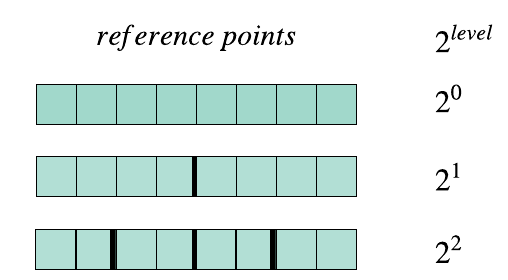
\includegraphics[width=0.4\textwidth]{pics/plot-figs/divtree4.png}
\caption{A demonstration of dividing the reference points at each node level.}
\label{fig:divtree}
\end{figure}

The completed tree will consist of the reorganised array of reference points, the original indices of the reference points and two arrays containing the dimensions with the widest spread and the median values, that together represent the splitting values of each node. In our optimised solution, the tree also consists of two 2D arrays containing the upper and lower bounds for each dimension at each current node. This idea is elaborated further in section \ref{sec:traversal}. 
\\[2mm]
The dimension with the widest spread is computed on lines 16-20, and subsequently, the values in that dimension are sorted, and the reference points and indices are gathered accordingly, on lines 21-24. The median value is picked out on line 25, and both the median and dimension are scattered into the tree arrays containing all medians and dimensions in lines 34-35. Since the upper and lower bounds are computed when finding the dimension with the widest spread, they too are scattered into the tree arrays containing all upper and lower bounds, in lines 36-37. 


\begin{listing}[H]
\begin{minted}{haskell}
entry buildTree [m][d] (points : [m][d]f32) (h: i32) =
    let num_pads =     (...)   -- computing the padding needed
    let padding  = map (...)   -- creating the padding array
    let reference = points ++ padding

    let (ref_idxs, reference, median_vals, median_dims, lower_bounds, upper_bounds) =
    	(...) -- initalising the loop variables
        for level < (h+1) do
            let num_nodes_pr_lvl = 1 << level
            let num_points_pr_node_pr_lvl = m // num_nodes_pr_lvl
            let reference = unflatten num_nodes_pr_lvl num_points_pr_node_pr_lvl reference
            let ref_inds  = unflatten num_nodes_pr_lvl num_points_pr_node_pr_lvl ref_idxs

            let (indices', reference', node_info', lower, upper) = unzip5 <|
                map3 (\i node_arr inds ->
                        let dim_arrs = transpose node_arr   |> intrinsics.opaque
                        let smallest = map o reduce         |> intrinsics.opaque
                        let largest  = map o reduce         -- max numbers for each dim
                        let differences = map         (...) -- computing differences
                        let (dim,_)     = reduce_comm (...) -- dimension w/ widest spread
                        let extract_dim = map         (...) -- extract dimension values
                        let d_sort_idxs = extract_dim |> sort |> map (.0)
                        let indices     = gather d_sort_idxs inds
                        let node_arrp   = gather2D d_sort_idxs node_arr
                        let median      = node_arrp[num_points_per_node_per_lvl // 2, dim]
                        let node_info   = (median, dim)
                        in (indices, node_arrp, node_info, smallest, largest)
                    ) (iota num_nodes_per_lvl) reference ref_inds

            let (medians, dims) = unzip node_info'
            let inds = map (...)   -- computing indices for scatter
            in (flatten ref_idxs', 
                flatten reference', 
                scatter median_vals inds medians,
                scatter median_dims inds dims, 
                scatter2D lower_bounds inds lower,
                scatter2D upper_bounds inds upper)

    in (ref_idxs, reference, median_vals, median_dims, lower_bounds, upper_bounds)
\end{minted}
\caption{Futhark implementation of the tree creation.}
\label{lst:tree}
\end{listing}

% \\[2mm]
% One essential optimisation of the k-d tree construction is the use of padding. Since the datasets might be of sizes that are not dividable with $2^{h+1}$, being the number of leaves, then padding the dataset to match the number of leaves, would allow regular parallelism which is much more efficient, since the parallel dimension will have the same size overall the elements of the map.
One essential optimisation of the k-d tree construction is the use of padding. Since the datasets might be of sizes that are not dividable with the number of leaves, then padding the dataset to match the number of leaves would mean the parallel dimension will have the same size overall the elements of the map, allowing regular parallelism and flattening, which is much more efficient.
\\[2mm]
% Assuming we choose a height that fits that dataset size, such that the number of points per leaf is in the hundreds, it is arguable that the proposed solution uses at most one padded element per leaf,  accounting to less than 1\% overhead. 
Arguably, the proposed solution uses at most one padded element per leaf, accounting to less than 1\% overhead. Assuming that we choose a height that fits that dataset size, such that the number of points per leaf is in the hundreds. 
% It is arguable that the proposed solution uses at most one padded element per leaf, and assuming that we choose a height that fits that dataset size, such that the number of points per leaf is in the hundreds, it accounts to less than 1\% overhead. 
\\[2mm]
The upper bound of the number of pads should not exceed the number of leaves, thus, we want to see how many pads that amount per leaf. 
In Equation \ref{eq:eq1} and \ref{eq:eq2} we denote $n$ to be the total number of reference points, $2^{h+1}$ computes the total number of leaves, where $h$ is the height of the tree excluding the leaves. Thus, $\ceil*{\dfrac{n}{2^{h+1}}}$ denotes the number of points per leaf. In Equation \ref{eq:eq1} we multiply the number of leaves with the number of points per leaf, we get the number of elements that are dividable with the total number of leaves, and by subtracting $n$, we will have the number of pads needed. In Equation \ref{eq:eq2} we divide with the number of leaves on each side, resulting in less than or equal to 1 pad per leaf. 

\begin{align} \label{eq:eq1}
% \textit{number of pads} \leq \textit{number}& \textit{ of leaves} \\[2mm]
\ceil*{\dfrac{n}{2^{h+1}}} \times 2^{h+1} - n   &\leq 2^{h+1} \\[2mm]
\ceil*{\dfrac{n}{2^{h+1}}} - \dfrac{n}{2^{h+1}} &\leq 1 \label{eq:eq2}
\end{align}


\subsubsection{Difficulties and Shortcomings}
\label{sec:treediff}
In the construct above in Listing \ref{lst:tree}, the original solution was to use a merge sort on line 19. However, although it was safe for Futhark to perform a loop distribution and loop interchange between the outer map inside both for loops, it did not realise, in which case the interchange was not performed. Thus, causing poor performance for the tree construction.  The solution was to (1) use batched merge sort, which operates on 2D arrays rather than 1D arrays, (2) distribute the map from line 12, across the body of the map function, such that the sorting is outside the map. 
\\[2mm]
Another shortcoming shows by the use of \texttt{intrinsics.opaque} at lines 14-15 in Listing \ref{lst:tree}, where the purpose is to prevent the Futhark compiler from fusing the two map-reduce compositions on lines 15-16. The reasoning behind this is that both map-reduce compositions call on the same size array, namely m. 
\\[2mm]
Since the Futhark compiler uses moderate flattening, a map-reduce composition will execute in parallel. However, in a map-reduce composition inside a map, as we have in lines 13 and 15-16, the inner map-reduce composition will be sequentialised, and thus resulting in inefficient code. By adding \texttt{intrinsics.opaque} and preventing the fusion, the compiler will create two reduce inside a map, which in return will exploit all parallelism. 


% 272512/256620 = 1,0619281428

% data/brute/10test-k3-d4.in
% [580000][4]f32


% with: 
% dataset data/traverse/13test-k3-d14.in: 97395033.00μs (avg. of 1 runs; RSD: 0.00)
% dataset data/traverse/13test-k5-d14.in: 108650237.00μs (avg. of 1 runs; RSD: 0.00)
% dataset data/brute/2brute2.in:       314551.00μs (avg. of 1 runs; RSD: 0.00)
% dataset data/brute/10test-k3-d4.in:  256620.00μs (avg. of 1 runs; RSD: 0.00)

% without:
% dataset data/traverse/13test-k3-d14.in: 97781445.00μs (avg. of 1 runs; RSD: 0.00)
% dataset data/traverse/13test-k5-d14.in: 108743904.00μs (avg. of 1 runs; RSD: 0.00)
% dataset data/brute/2brute2.in:       319978.00μs (avg. of 1 runs; RSD: 0.00)
% dataset data/brute/10test-k3-d4.in:  272512.00μs (avg. of 1 runs; RSD: 0.00)














% In the construct above in listing \ref{lst:tree}, if we look only at the construct between the \texttt{map3} on line 12 and the merge sort performed on line 19, we would get the following structure.
% if we look only at the construct between the \texttt{map3} on line 12 and the merge sort performed on line 19, we would get the following structure.
% \begin{verbatim}
% 	map 
% 	    for i < d
% 	        for j < i+1
% 	            map f (size n)
% \end{verbatim}

% 	We need to make sure that we are not reversing any of the direction vectors. It cannot start with < (greater than). 

% 	If the outer loop is parallel - then we can interchange always. 

% 	A parallel loop can always be interchanged inside (meaning inwards) - expect in the cases in which the loop index or loop bounds depend on that parallel loop index or on the map. 

% What you would like to do with this code is to interchange the outer map inside both for loops, and then we will have: 
% 	for
% 		for
% 			map
% 				map

% and then we can flatten the two maps and that's done at this point because you have two perfectly nested maps. 


% Fixed by using batched merge sort -> instead of operating on a 1D array we operate on a 2D array, the idea is to distribute the map and you distribute the map across the body of the map function such that you separate the sorting part of it from the rest. 

% So the sorting is outside the original outer map. 

% 	map
% 		map
% 		sort
% 		map

% -> parallel loop distribution and loop interchange. This is what gives you easy flattening for regular cases which is what Futhark s doing. But in this case Futhark is stupid, because it doesn't realise that the inner loop for j ... , since that the bound is i+1 -> it thinks that it cannot interchange the outer map. So it's a Futhark limitation. 


















% \begin{listing}[H]
% \begin{minted}{haskell}
% entry buildTree [m][d] (imB : [m][d]f32) (h: i32) =
%     let num_nodes  = (1 << (h+1)) - 1
%     let num_leaves =  1 << (h+1)
%     let ppl  = (m + num_nodes) / num_leaves  -- ceil(m / (2^(h+1)))
%     let m'   = ppl * num_leaves
%     let num_pads = m' - m
%     let pad = map (\_ -> map (\_ -> f32.inf) (iota d)) (iota num_pads)
%     let imB = imB ++ pad
%     let num_patches_in_leaf = m' // num_leaves
%     let tot_nodes = num_nodes+num_leaves

%     let (ref_idxs, reference, median_vals, median_dims, lower_bounds, upper_bounds) =
%         loop(ref_idxs, reference, median_vals, median_dims, lower_bounds, upper_bounds) =
%           (iota m, points, replicate..., replicate..., replicate..., replicate...)

%         for level < (h+1) do
%             let num_nodes_per_lvl = 1 << level
%             let num_points_per_node_per_lvl = m // num_nodes_per_lvl

%             let (imB_idxs', reference, node_info', lower, upper) = unzip5 <|
%                 map3 (\i node_arr inds ->
%                         let dim_arrs = transpose node_arr   |> intrinsics.opaque
%                         let smallest = map o reduce         |> intrinsics.opaque
%                         let largest  = map o reduce
%                         let differences = map (...) 	-- computing differences
%                         let (dim,_)     = reduce (...)  -- dimension w/ widest spread
%                         let extract_dim = map (...) 	-- extract dimension values
%                         let d_sort_idxs = extract_dim |> sort |> map (.0)
%                         let indices     = gather d_sort_idxs inds
%                         let node_arrp   = gather2D d_sort_idxs node_arr
%                         let median      = node_arrp[num_points_per_node_per_lvl // 2, dim]
%                         let node_info   = (median, dim)
%                         in (indices, node_arrp, node_info, smallest, largest)

%                     ) (iota num_nodes_per_lvl) referencep ref_inds

%             let test = ref_idxs'
%             let (medians, dims) = unzip node_info'

%             let inds = map (...)
%             in (flatten ref_idxs', flatten reference, scatter median_vals inds medians,
%                 scatter median_dims inds dims, scatter2D lower_bounds inds lower,
%                 scatter2D upper_bounds inds upper)

%     in (ref_idxs, reference, median_vals, median_dims, lower_bounds, upper_bounds)
% \end{minted}
% \caption{Futhark implementation of the tree creation.}
% \label{lst:tree}
% \end{listing}


















\subsection{Tree Traversal}
\label{sec:traversal}
% At each step you reason about tradeoffs/alternative design choices and
% justify why you did it in the way you did it (advantages/shortcommings,
% and why your approach is reasonable). Of course mostly related to performance.

% Whenever possible, support your reasoning with (as in point to) experimental
% evaluation results (next).

% \begin{itemize}
% 	\item using an integer to represent the stack
% 	\item the first traversal logic (show figure)
% 	\item the continuous traversal logic (show figure)
% 	\item checking a median on one dimension
% 	\item checking all medians from all dimensions (show equation)
% 	\item 
% 	\item 
% 	\item 
% \end{itemize}	

%   3.3 Tree Traversal
%     - explaining the solution to use a stack 
%     - showing a figure of the first traversal: first go to the leaf in which the query naturally belongs, there is a unique leaf to which it naturally belongs to 
%     - showing (2-3) figures of the continuous traversal with a stack

%     3.3.1 Representing the Stack as an Integer
%       - including an equation that shows the bit arithmetic of setVisited

%     3.3.2 Validating Whether to Look at the `second`
%       - reasoning about the original median check
%       - showing and reasoning about Cosmin's equation
%       - comparing the two
%         - benefits, trade-offs


% As mention in the Background, Futhark does not support recursion, which is why the pseudo-code from Algorithm 3 is rewritten into an imperative version. One such solution is using a stack to traverse the tree incrementally while deciding which nodes to visit next. The figure below demonstrates the traverse down to the first leaf; this example does not need a stack because, at this point, we do not know if we need to visit additional leaves. Figures X-X show the traversal continuing from the first leaf, in which a stack is necessary. 
% Divide and conquer recursion is difficult to map, especially efficiently for parallel execution. Due to divergence and various irregular things.  



In section \ref{sec:back} the tree traversal Algorithm \ref{alg:tree}, is created using recursion, and as in section \ref{sec:kdtree} we must re-write the traversal without recursion. The proposed solution uses a stack, and the stack is represented as an integer, since the height of the tree never exceeds 32. 
\\[2mm]
The traversal has two stages overall stages: (1) the first traversal finding the unique leaf in which the query naturally belongs, (2) backtracking the tree to find additional or better KNNs. 

\subsubsection{The First Traversal}

As described in section \ref{sec:back}, first denotes the child of the current node that is on the same side as median w.r.t the query, similarly second denotes the child of the current node that is on the opposite side of the median. 
Figure \ref{fig:t1} demonstrates how the tree is traversed to the leaf in which the query belongs, note that the leaf marked with red is denoted first and its sibling leaf is denoted second. 

\begin{figure}[H]
\centering
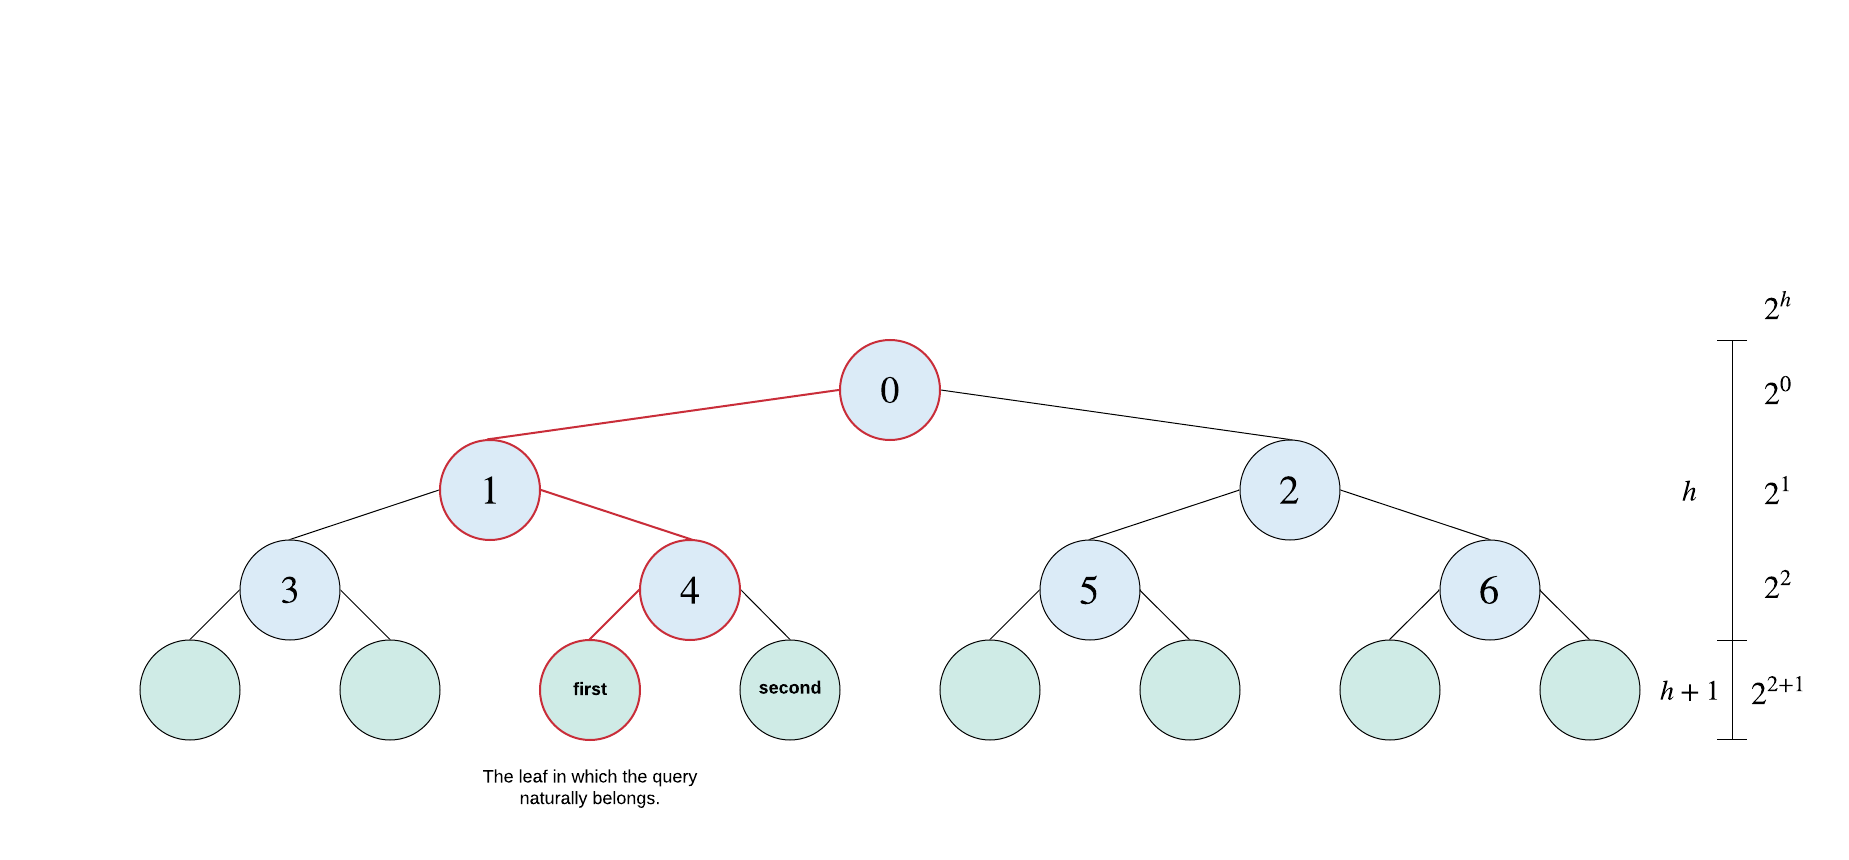
\includegraphics[width=1\textwidth]{pics/kd-tree-visual/22.png}
\caption{The first traversal finding the leaf in which the query naturally belongs.}
\label{fig:t1}
\end{figure}

% \begin{listing}[H]
% \begin{minted}{haskell}
% entry firstTraverse [d][q] (height:   i32)  (median_dims: [q]i32)
%                            (query: [d]f32)  (median_vals: [q]f32) =

%     let new_leaf = loop node_index = 0
%         while !(isLeaf height node_index) do
%           if query[median_dims[node_index]] <= median_vals[node_index]
%           then (node_index+1)*2-1
%           else (node_index+1)*2

%     in new_leaf
% \end{minted}
% \caption{Futhark implementation of the first tree traversal.}
% \label{lst:first}
% \end{listing}


\subsubsection{The Traversal for Additional Leaves}


In this demonstration, we look at a fictive traversal in which we always check the second node. The validation technique as to whether to check the second node or not, is elaborated in section \ref{sec:valid}. 
\\[2mm]
Figure \ref{fig:t2} is a continuation of figure \ref{fig:t1}, in which the initial leaf is reached and the stack is popped to see if the second node has been visited or not. Since it had not been visited, the traversal also visits the second node. 

% \begin{figure}[H]
% \centering
% 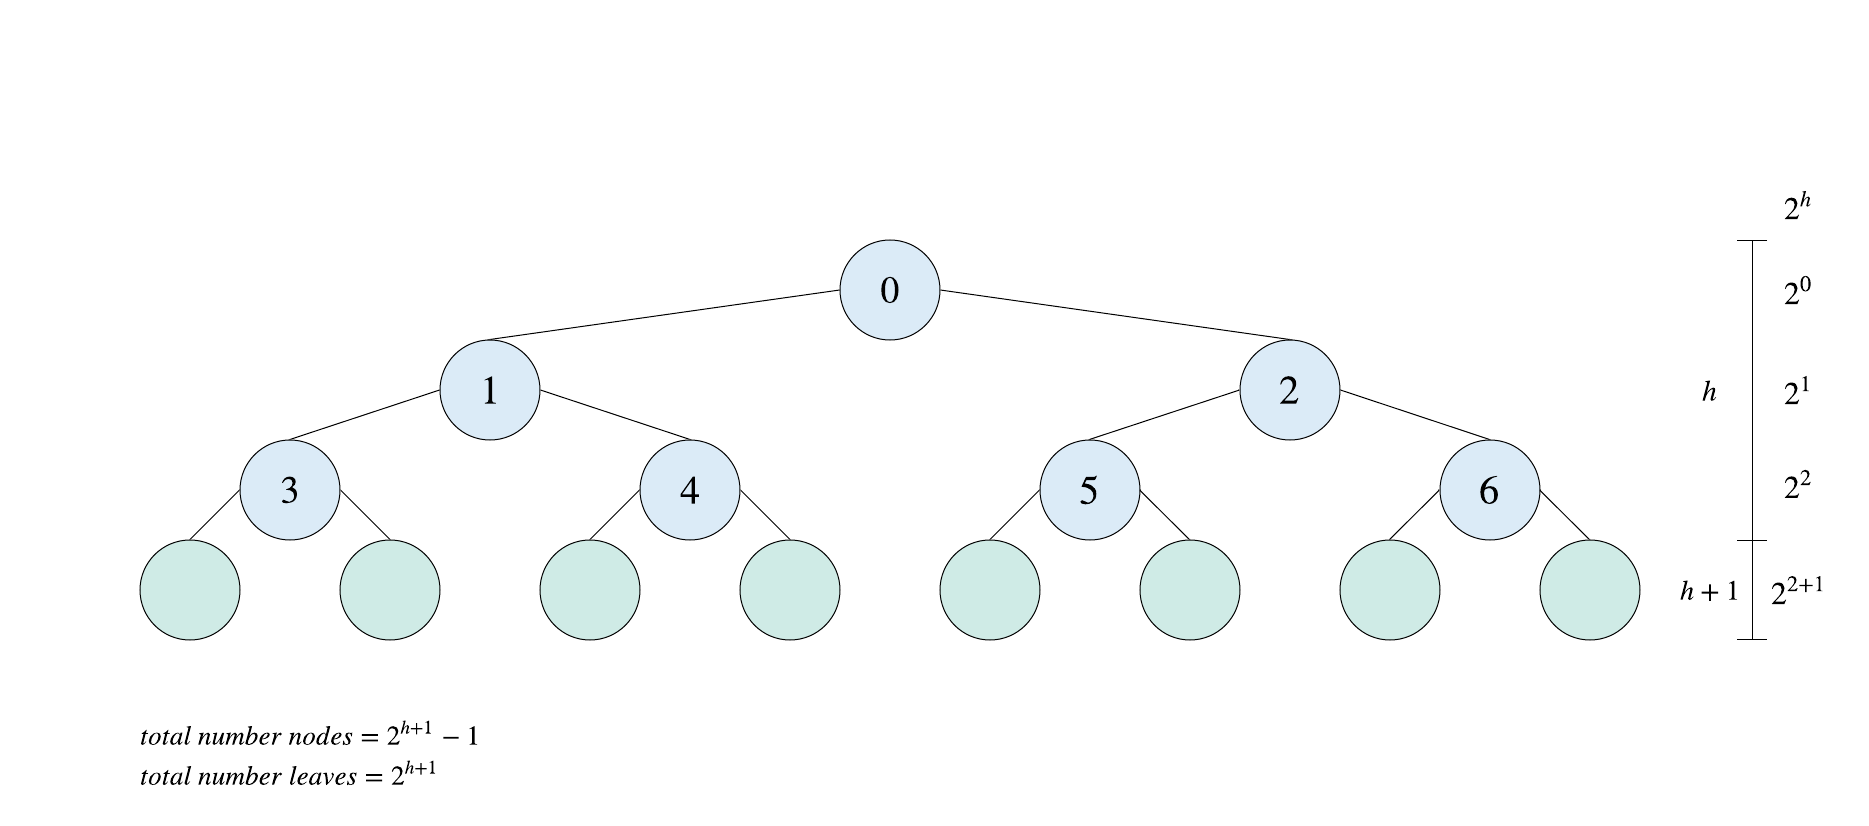
\includegraphics[width=0.9\textwidth]{pics/kd-tree-visual/1.png}
% \caption{}
% \end{figure}


% \begin{figure}[H]
% \centering
% 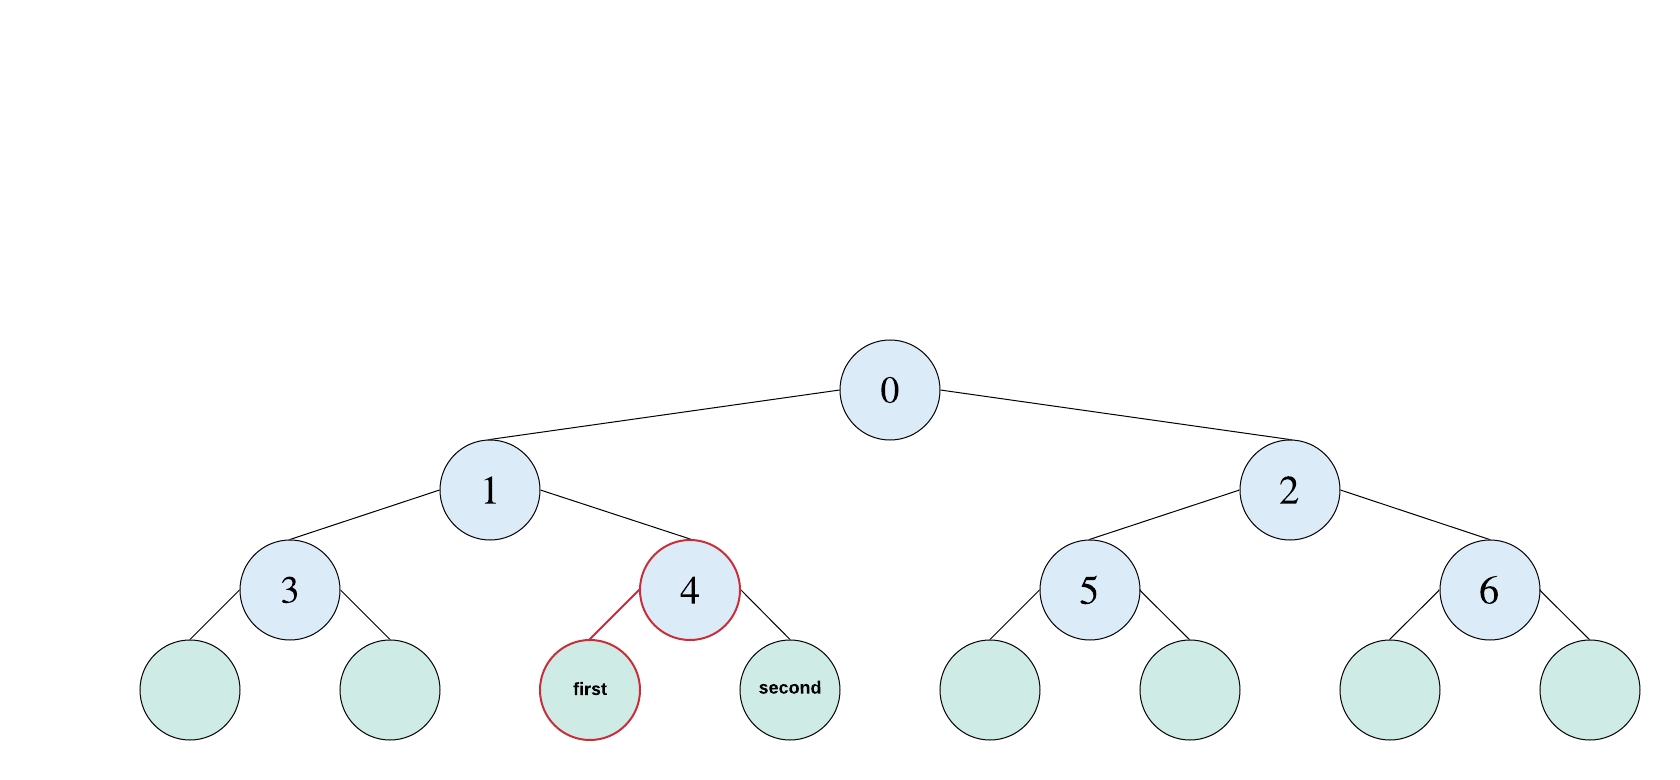
\includegraphics[width=0.9\textwidth]{pics/kd-tree-visual/3.png}
% \caption{}
% \end{figure}

% \begin{figure}[H]
% \centering
% 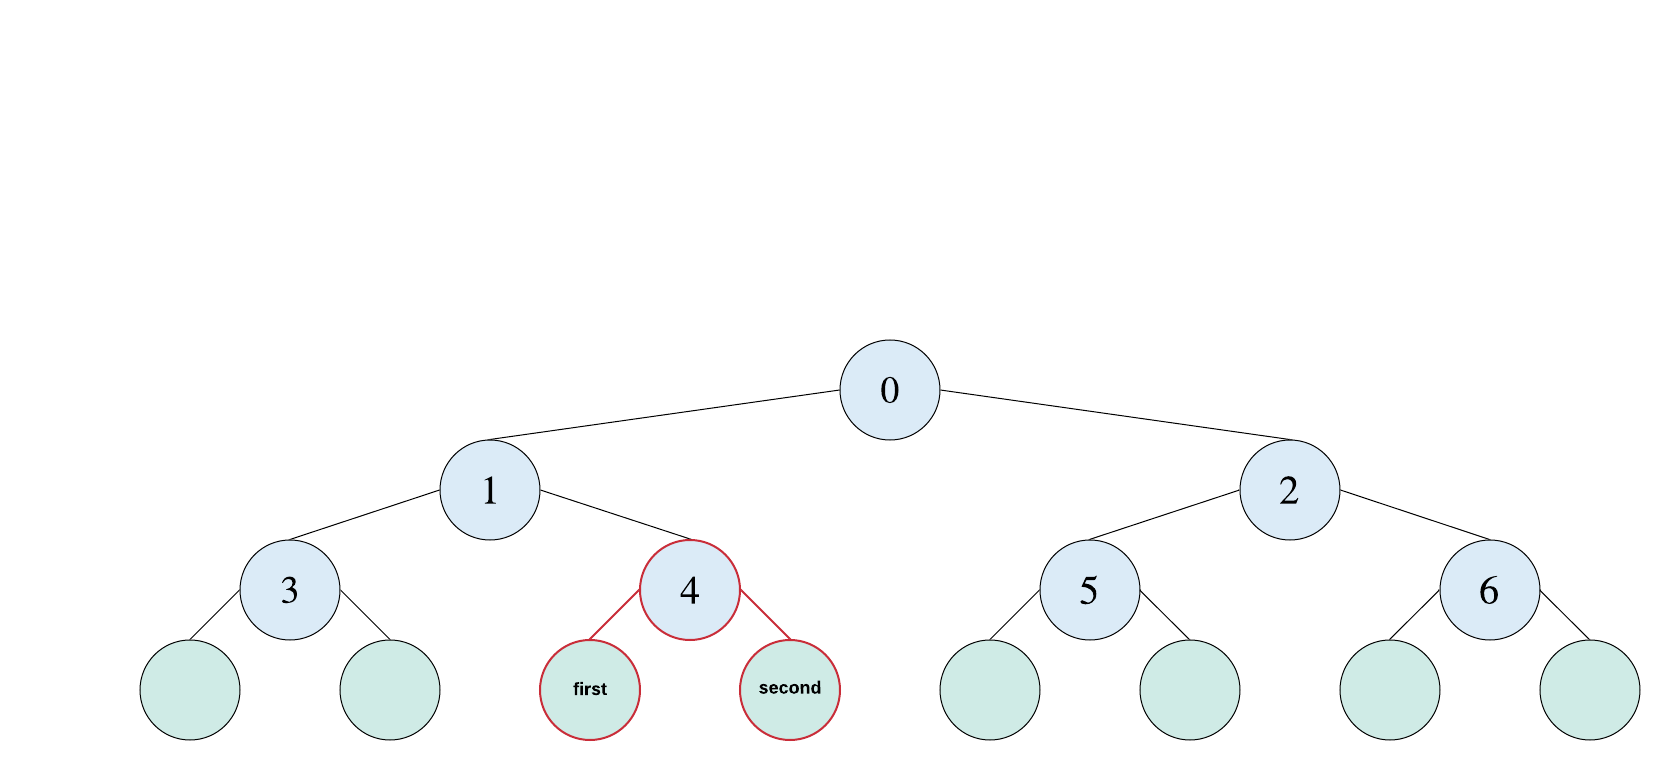
\includegraphics[width=0.9\textwidth]{pics/kd-tree-visual/4.png}
% \caption{}
% \end{figure}

\begin{figure}[H]
\centering
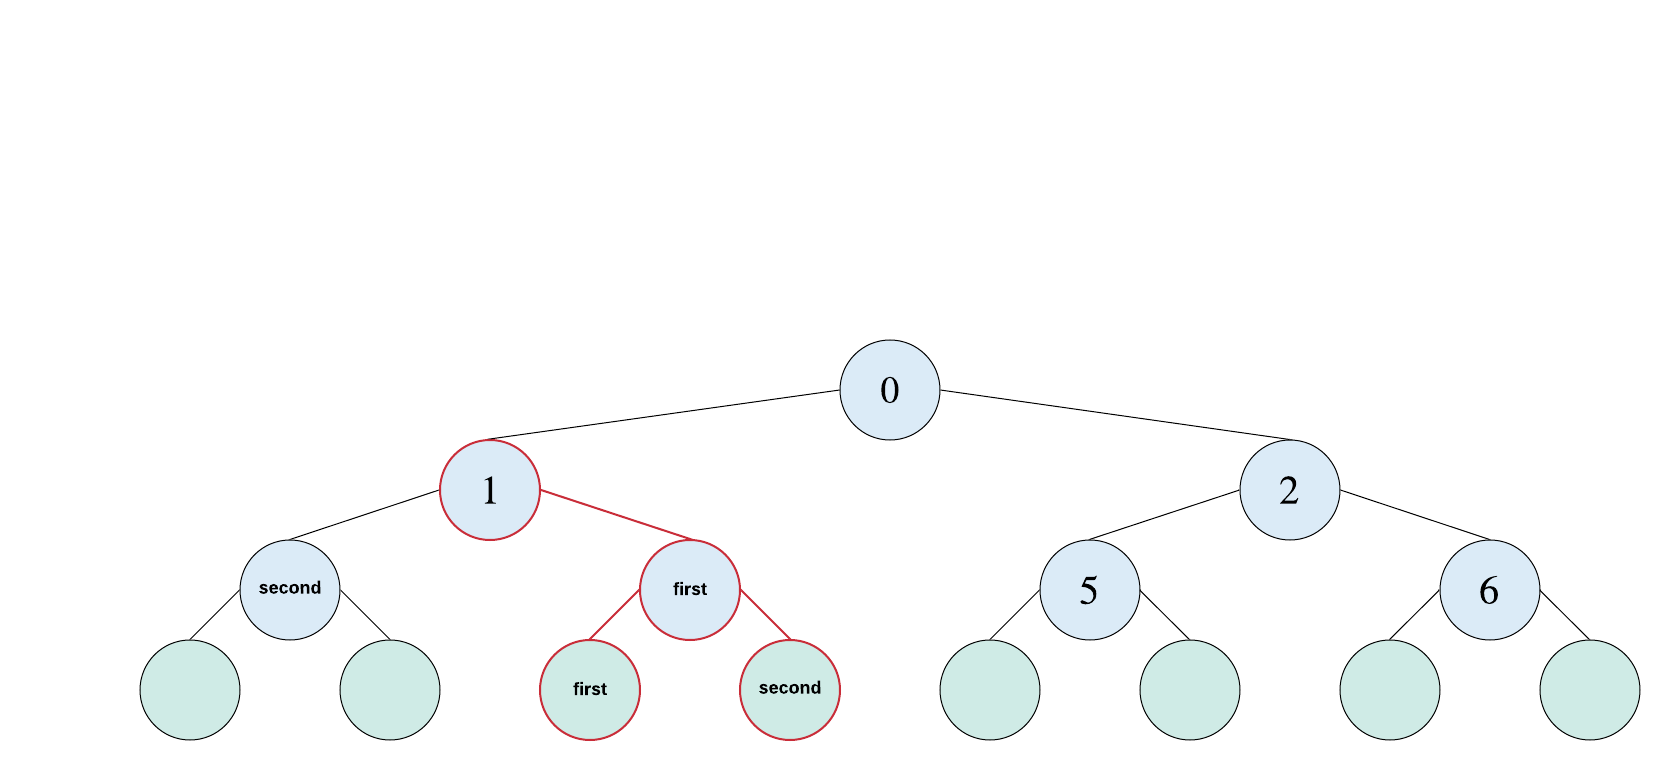
\includegraphics[width=0.9\textwidth]{pics/kd-tree-visual/5.png}
\caption{Visiting the second node of the initial leaf.}
\label{fig:t2}
\end{figure}

\noindent In figure \ref{fig:t3} the traversal looks to the parents second child, and since that has not yet been visited, it traverses to the first leaf of the parents second child.  

% \begin{figure}[H]
% \centering
% 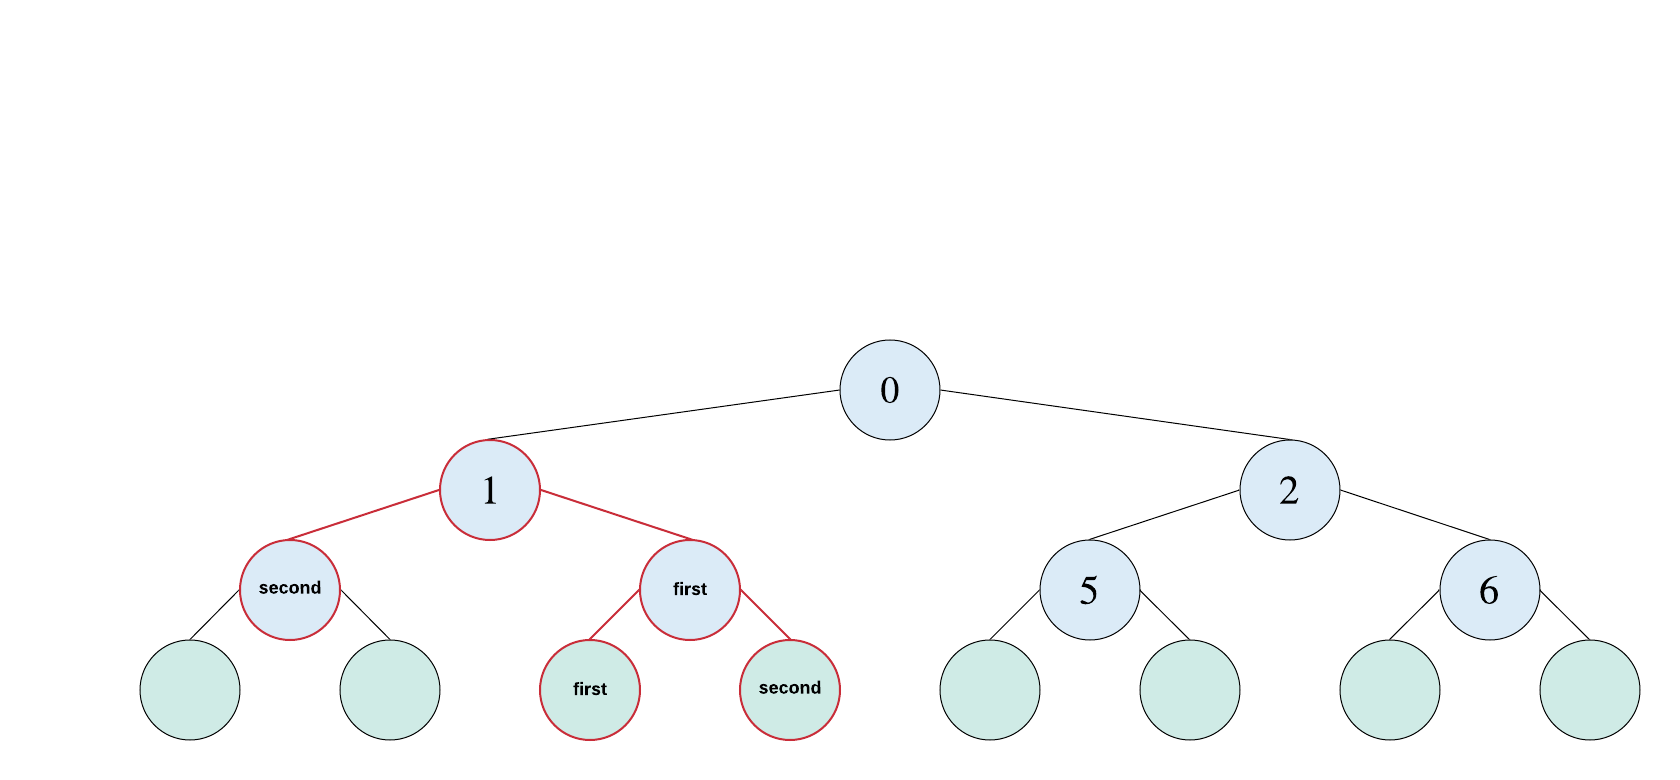
\includegraphics[width=0.9\textwidth]{pics/kd-tree-visual/6.png}
% \caption{}
% \end{figure}

\begin{figure}[H]
\centering
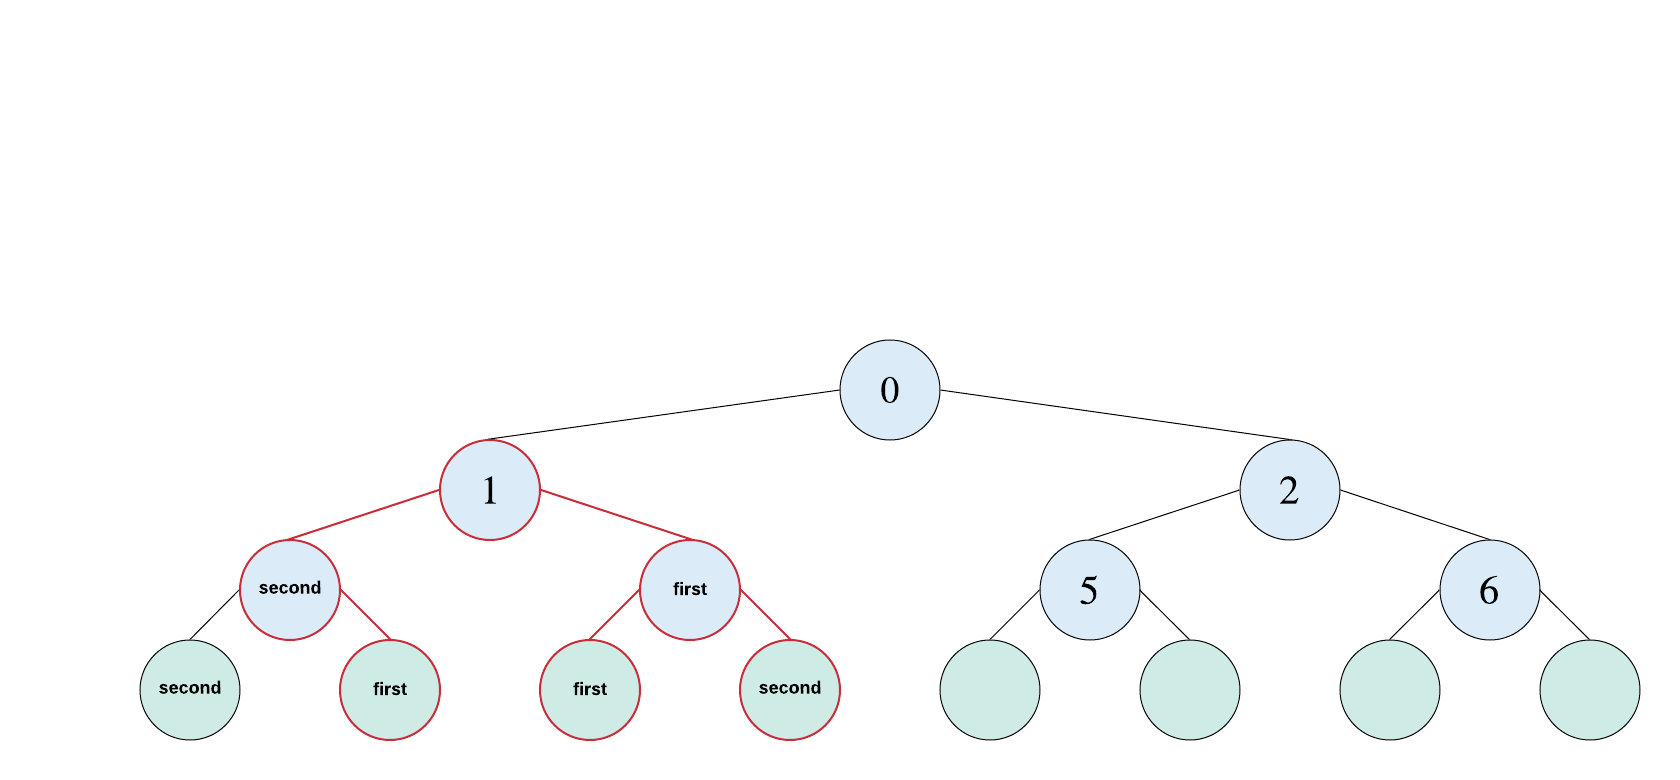
\includegraphics[width=0.9\textwidth]{pics/kd-tree-visual/7.png}
\caption{Visiting first node of the parents second child.}
\label{fig:t3}
\end{figure}

\noindent Pretending that we still have not found the KNN, the traversal will continue into the second leaf of the parents second child, as in figure \ref{fig:t5}. If the KNN is still not found, the traversal will continue to the second child of the root until the whole tree has been traversed, or the KNN is found. 

% \begin{figure}[H]
% \centering
% 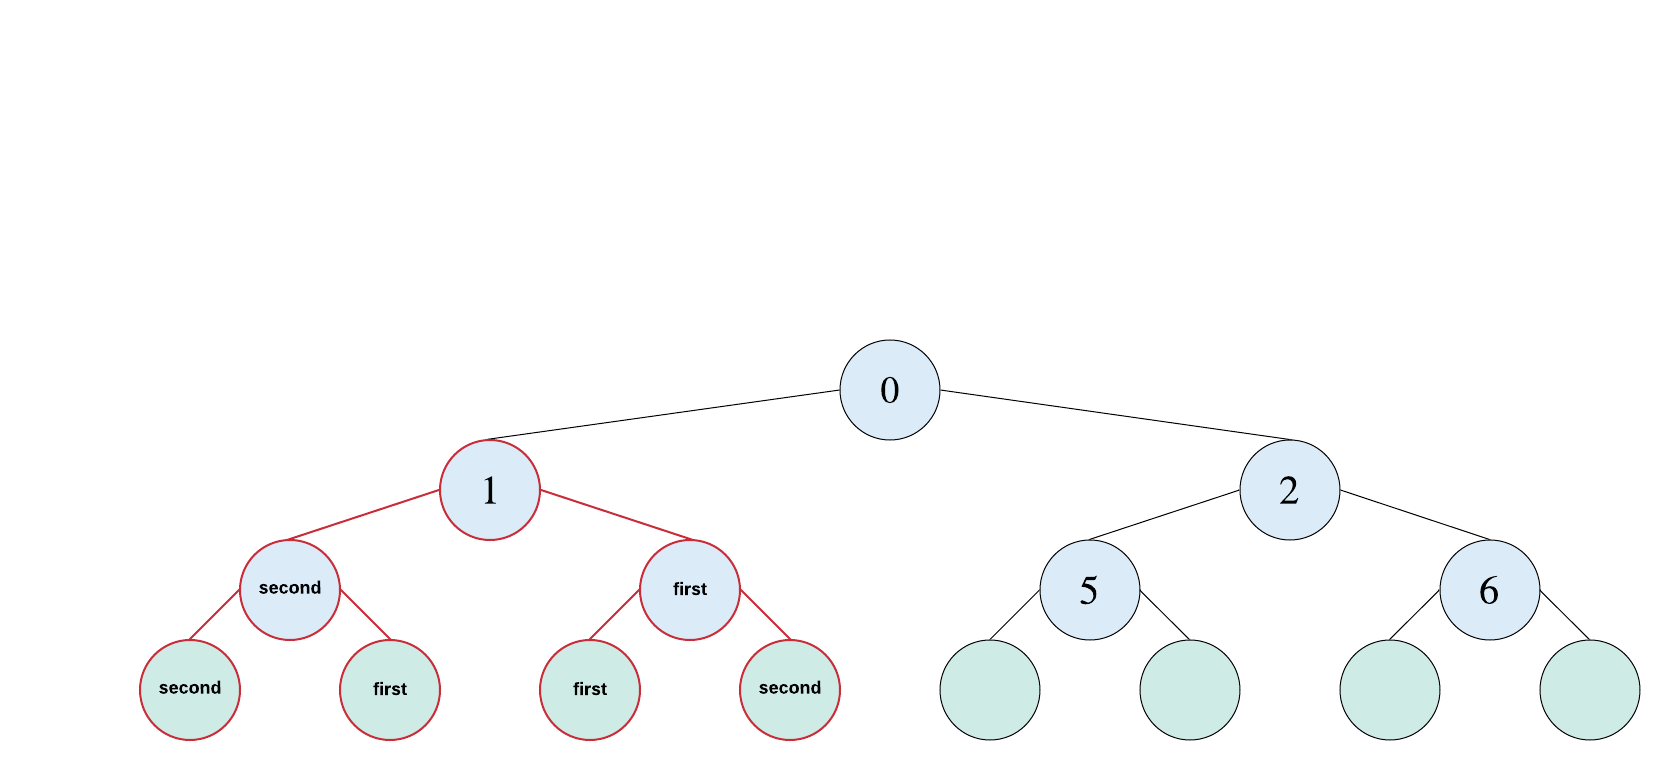
\includegraphics[width=0.9\textwidth]{pics/kd-tree-visual/8.png}
% \caption{}
% \end{figure}

% \begin{figure}[H]
% \centering
% 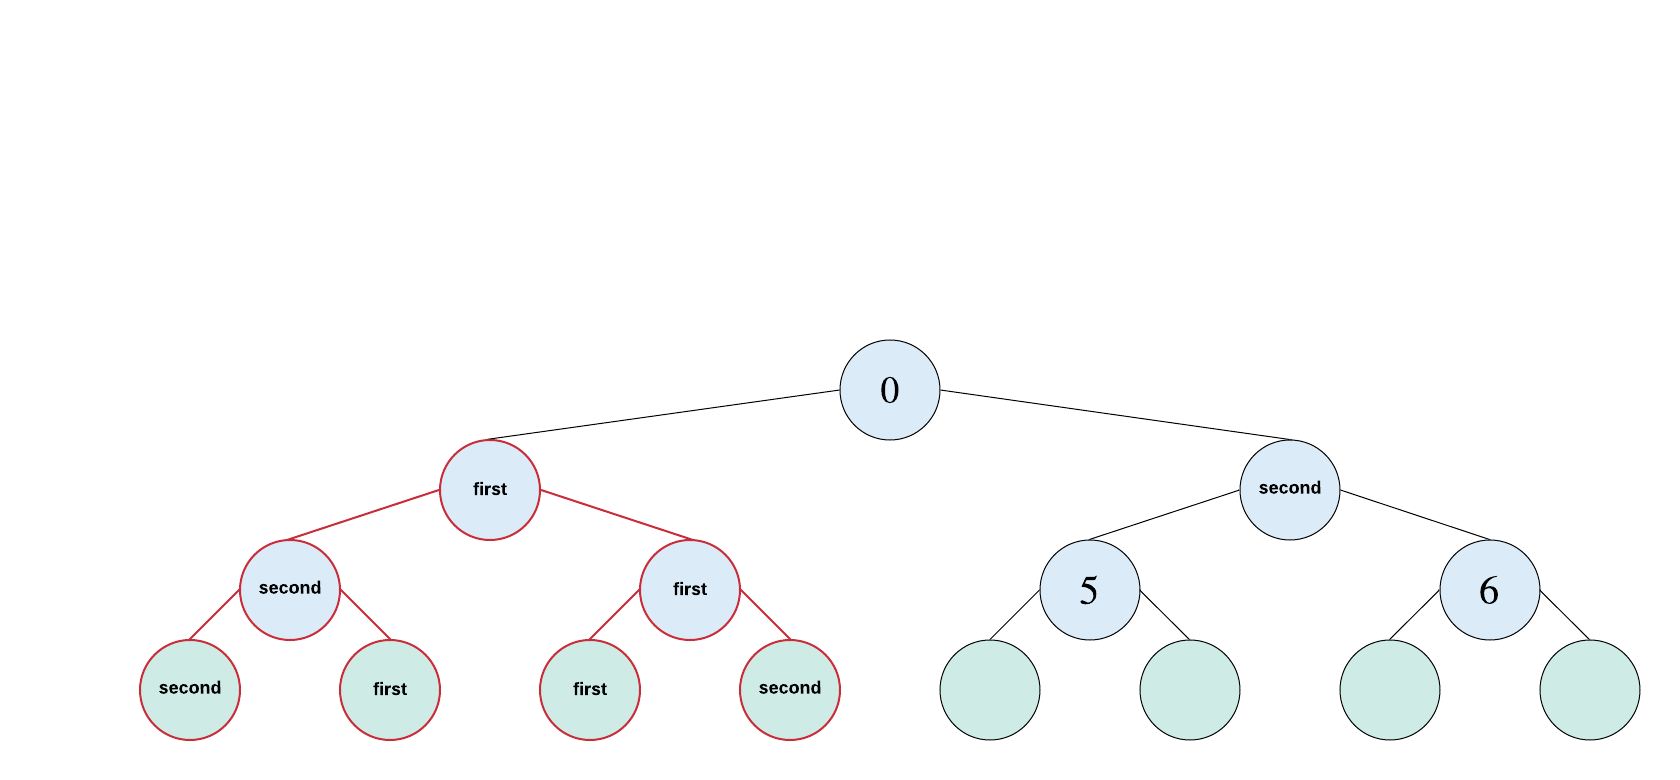
\includegraphics[width=0.9\textwidth]{pics/kd-tree-visual/9.png}
% \caption{}
% \end{figure}

% \begin{figure}[H]
% \centering
% 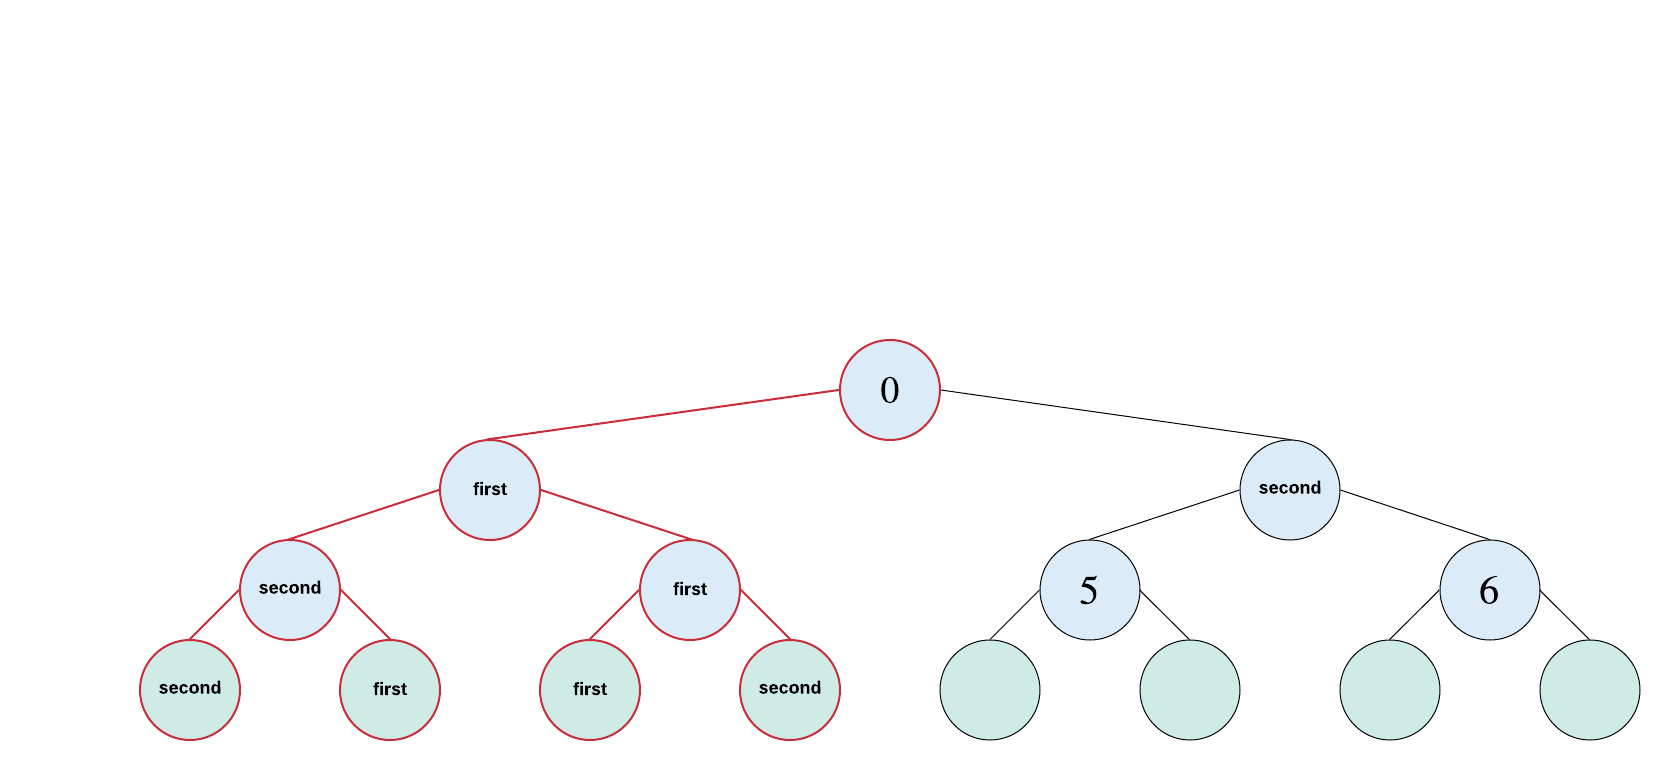
\includegraphics[width=0.9\textwidth]{pics/kd-tree-visual/10.png}
% \caption{}
% \label{fig:t4}
% \end{figure}

\begin{figure}[H]
\centering
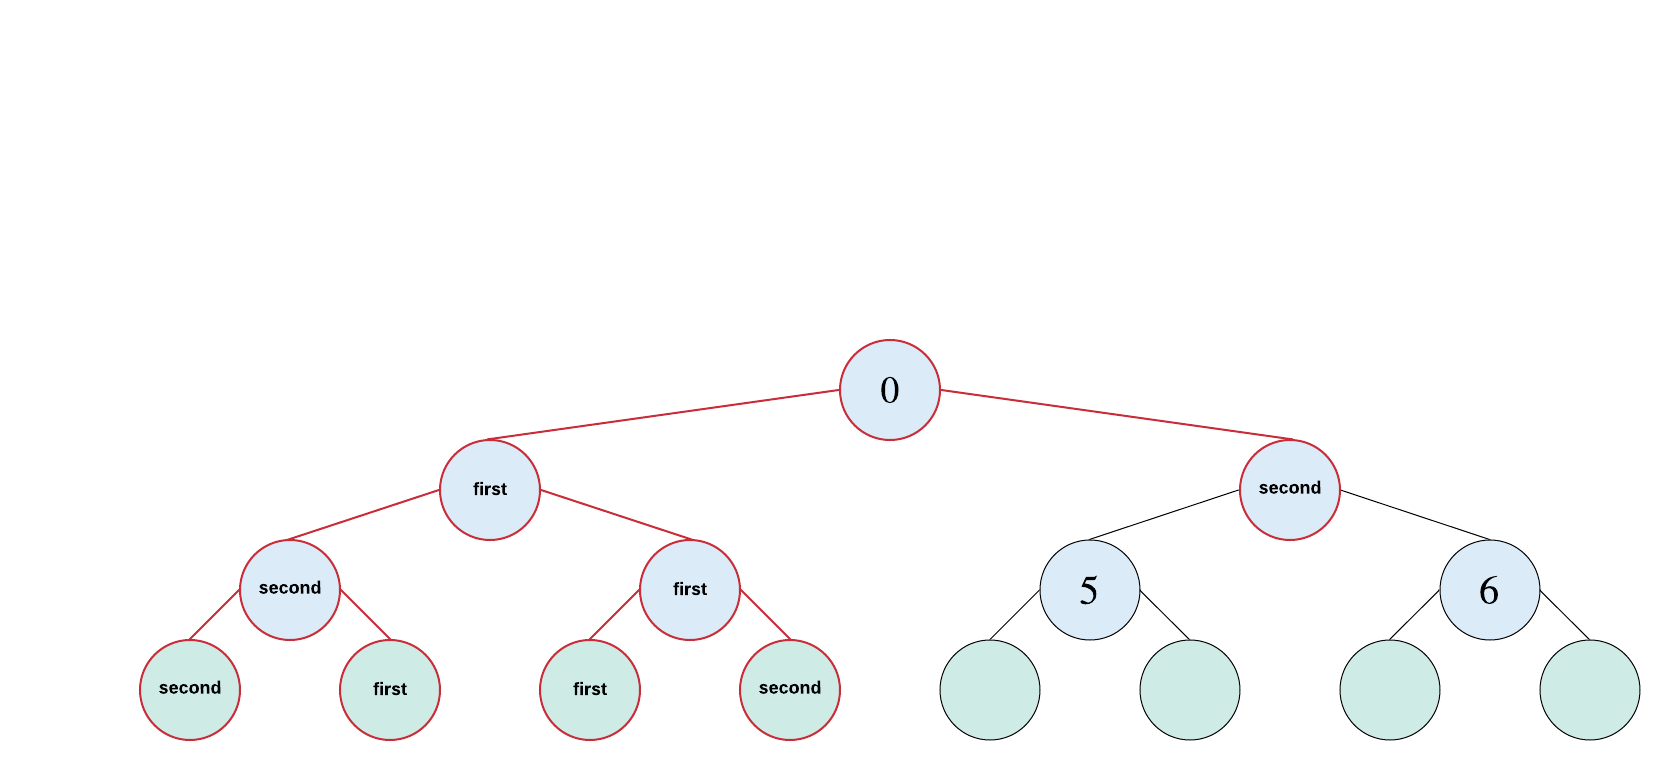
\includegraphics[width=0.9\textwidth]{pics/kd-tree-visual/11.png}
\caption{}
\label{fig:t5}
\end{figure}




% \subsubsection{Representing the Stack as an Integer}

%The naive solution of representing a stack is using a boolean list where the leaves and node are set to true once visited. Although this is a simple and correct solution, 
% The stack is represented as an integer, since the height of the tree never exceeds 32, making it is plausible. 
%it can be further optimised as an integer representation instead. % The code in listing XX shows the bit arithmetic done to modify the right areas of the stack and the logic behind setVisited is demonstrated in XX. 

% \begin{listing}[H]
% \begin{minted}{haskell}
%   let setVisited (stk: i32) (c: i32) : i32 =
%       stk | (1 << c)
%   let resetVisit (stk: i32) (c: i32) : i32 =
%       stk & !(1 << c)
%   let isVisited (stk: i32) (c: i32) : bool =
%       (stk & (1 << c)) > 0i32
% \end{minted}
% \caption{Snippet of bit arithmetic for stack modifications.}
% \label{lst:stack}
% \end{listing}

% \begin{figure}\label{fig:bits}
% \begin{align*}
%   && &00000000000000000000100010000101 &\\ \text{or} 
%   && &00000000000000000000001000000000 &\\ 
%   \cline{3-4}
%   && &00000000000000000000101010000101
% \end{align*}
% \caption{Example of stack integer arithmetic.}
% \end{figure}



% \begin{align*}
%   && &00000000000000000000101010000101 &\\ \text{and} 
%   && &11111111111111111111110111111111 &\\ 
%   \cline{3-4}
%   && &00000000000000000000100010000101
% \end{align*}







\subsubsection{Validating Whether to Look at the \texttt{second}}
\label{sec:valid}

We propose an optimised solution for checking whether to visit the second node or not. $wknn$ denotes the worst found neighbour so far, $R$ denotes our reference points, $Q$ denotes our queries, $lb$ and $ub$ denote the arrays containing the upper and lower bounds and $M$ denotes the array containing the median values for each node. 

\[
\forall i.[lb_i, ub_i].\ \forall q\in Q_m.\ \forall p\in R_n.\ \forall m\in M_{nn}.
\]

\noindent The original solution determines whether to visit the second node by checking if the distance from the query to the current median is smaller than the worst found neighbour, as in Equation \ref{eq:e1}. However, the solution looks only at one dimension when checking whether to visit or not, meaning that it is likely that another dimensionality could contain information that would otherwise have prevented the second visit. Especially if the number of dimensions is, because then a lot of values will be overlooked. 
% The original solution looks at one dimension when checking whether to visit the second node or not.

\begin{equation}  \label{eq:e1}
\mid q_i - m_i \mid\ >\ wknn
\end{equation} 

\noindent The naive approach would be to compute all distances, as in Equation \ref{eq:e2}. Although this has a higher level of accuracy compared to the original solution, it also inefficient. 

\begin{equation}  \label{eq:e2}
% \substack{ \forall i.[lb_i, ub_i]. \\ \forall q\in Q_m. \\ \forall p\in R_n.} \ 
\sqrt{ \sum_{i}^{} (p_i - q_i)^2  }
\ \geq\ wknn
\end{equation}

\noindent Instead, we propose a solution that achieves a higher level of accuracy compared to the original solution, while still running efficiently. The idea is that the upper and lower bounds for each dimension is saved, for each node, and then used to compute the distance between the query to the upper and lower bounds, respectively. Thus, instead of checking one dimension, we check all dimensions, but only against the upper and lower bounds. This is formulated in Equation \ref{eq:e3} and it corresponds to lines 11-26 in Listing \ref{lst:traverse1}. 

\begin{equation}  \label{eq:e3}
% \substack{ \forall i.[lb_i, ub_i]. \\ \forall q\in Q_m. \\ \forall p\in R_n.} \ 
\sqrt{ \sum_{i}^{} (p_i - q_i)^2  }\ \geq\
\sqrt{\sum_{i}^{} \substack{(q_i-lb_i)^2 \\ (q_i-ub_i)^2 \\\text{  ~ ~ ~   }0}  \substack{\text{, if  ~ } q_i\ \leq\ lb_i \\ \text{, if  ~ } q_i\ \geq\ ub_i \\\text{, ~ otherwise} }}
\ \geq\ wknn
\end{equation}

\noindent Section \ref{sec:evaltrav} demonstrates the increased performance by using this solution. On a dataset of size roughly 4 mio., with dimensionality D=12 and K=5, we obtain a speed-up of $5.6$. The reason for this is elaborated further in Section \ref{sec:evaltravhist}, which demonstrates how the checking all the upper and lower bound on all dimensions reduces the number of visits to additional node, due to its increased accuracy. Thus, reducing the steps made in the traversal and improving the performance. 


\begin{listing}[H]
\begin{minted}{haskell}
  let (parent_rec, stack, count, rec_node) =
      loop (node_index, stack, count, rec_node) =
           (last_leaf, stack, height, -1)
            while (node_index != 0) && (rec_node < 0) do
                let parent = getParent node_index
                let second = node_index + addToSecond node_index in

                if isVisited stack count
                then (parent, stack, count-1, -1)
                else
                  let ack = loop ack = 0.0f32
                      for i < d do
                          let cur_q = query[i]
                          let lower = lower_bounds[second,i]
                          let upper = upper_bounds[second,i] in

                          if cur_q <= lower then
                              let res = (cur_q-lower)*(cur_q-lower)
                              in (ack + res)
                          else if cur_q >= upper then
                              let res = (cur_q-upper)*(cur_q-upper)
                              in (ack + res)
                          else (ack + 0.0)

                  let to_visit = (f32.sqrt ack) < wknn in
                  if !to_visit
                  then (parent, stack, count-1, -1)
                  else
                    let second = node_index + addToSecond node_index
                    let stack  = setVisited stack count in
                    (parent, stack, count, second)
\end{minted}
\caption{A part of the tree traversal demonstrating checking upper and lower bound to determine visits.}
\label{lst:traverse1}
\end{listing}


% \[
%   \sum_{i}^{} \substack{(q_i-lb_i)^2, if  q_i \leq lb_i \\ (q_i-ub_i)^2, if  q_i \geq ub_i \\0 , otherwise }
% \]

% \begin{equation}
%   \sqrt{\sum_{i}^{} \substack{(q_i-lb_i)^2 \\ (q_i-ub_i)^2 \\\text{  ~ ~ ~   }0 }  \substack{\text{, if  ~ } q_i\ \leq\ lb_i \\ \text{, if  ~ } q_i\ \geq\ ub_i \\\text{, ~ otherwise} }}
% \end{equation}

% \[
%   \sum_{\substack{i=0 \\ i\neq 4}}^n \substack{i=0 \\ i\neq 4}
% \]


% \[
% \mathit{dist} = 
% \sqrt{ \left( \frac{dx}{hx} \right)^{\!\!2} +  \left( \frac{dy}{hy} \right)^{\!\!2} +  \left( \frac{dz}{hz} \right)^{\!\!2}}
% \]


% \begin{listing}[H]
% \begin{minted}{haskell}
% entry traverse [d][n][l] (height:             i32)  (median_dims:     [n]i32)
%                          (median_vals:     [n]f32)  (wknn:               f32)
%                          (query:           [d]f32)  (stack:              i32) 
%                          (last_leaf:          i32)  (lower_bounds: [l][d]f32)
%                          (upper_bounds: [l][d]f32)  : (i32, i32) =

%   (...) -- stack functions for checking and setting the stack

%   let (parent_rec, stack, count, rec_node) =
%       loop (node_index, stack, count, rec_node) =
%            (last_leaf, stack, height, -1)
%             while (node_index != 0) && (rec_node < 0) do
%                 let parent = getParent node_index
%                 let second = node_index + addToSecond node_index in

%                 if isVisited stack count
%                 then (parent, stack, count-1, -1)
%                 else
%                   let ack = loop ack = 0.0f32
%                       for i < d do
%                           let cur_q = query[i]
%                           let lower = lower_bounds[second,i]
%                           let upper = upper_bounds[second,i] in

%                           if cur_q <= lower then
%                               let res = (cur_q-lower)*(cur_q-lower)
%                               in (ack + res)
%                           else if cur_q >= upper then
%                               let res = (cur_q-upper)*(cur_q-upper)
%                               in (ack + res)
%                           else (ack + 0.0)

%                   let to_visit = (f32.sqrt ack) < wknn in
%                   if !to_visit
%                   then (parent, stack, count-1, -1)
%                   else
%                     let second = node_index + addToSecond node_index
%                     let stack  = setVisited stack count in
%                     (parent, stack, count, second)

%   let (new_leaf, stack, _) =
%       if parent_rec == 0 && rec_node == -1 then
%            (-1, stack, 0)

%       else loop (node_index, stack, count) =
%                 (rec_node, stack, count)
%            while !(isLeaf height node_index) do
%               let count = count + 1
%               let stack = resetVisit stack count in
%               if query[median_dims[node_index]] <= median_vals[node_index]
%               then ((node_index+1)*2-1, stack, count)
%               else ((node_index+1)*2, stack, count)

%   in (new_leaf, stack)
% \end{minted}
% \caption{Futhark implementation of the tree traversal.}
% \label{lst:traverse}
% \end{listing}





% \subsubsection{Difficulties and Shortcomings}








































\subsection{The Full Implementation}
\label{sec:full}
% At each step you reason about tradeoffs/alternative design choices and
% justify why you did it in the way you did it (advantages/shortcommings,
% and why your approach is reasonable). Of course mostly related to performance.

% Whenever possible, support your reasoning with (as in point to) experimental
% evaluation results (next).

% 3.4 The Full Implementation
%       - explain how things are put together - main function
%       - reason about sorting the queries by the leaves - why is it faster? optimises locality of reference, temporal locality because by sorting the queries by the leaves the same leaves are accessed in order. 


Listing \ref{lst:full} shows, in pseudo-code, the overall structure of the main function that puts all parts together. We experiment with two solutions for splitting the queries that have found their KNN, with the ones that need to continue traversing the tree. The first solution is using the two-way partition, elaborated further in section \ref{sec:pard}. The second solution is to sort the queries by the leaves, and this is elaborated further in section \ref{sec:sord}. 
\\[2mm]
The structure of Listing \ref{lst:full} is as follows. The first step is building the tree of the reference points, on line 3. The second step is to perform the first traversal for each query to the leaves in which the queries naturally belong, on line 4. The third step is a sequential outer while-loop, on lines 12-37, which continues to iterate until all queries have found their KNN. 
\\[2mm]
Inside this loop, we have a parallel map which performs two main tasks, (1) performing brute force on each ongoing query with its current leaf, in line 19, and (2) traversing the tree to find new leaves for the ongoing queries, on line 21. 
\\[2mm]
On lines 25-29, we either sort or partition the completed queries, from the non-completed queries. Since both partition and sorting reorganise the contents of the arrays, they do not change the sizes of them. Thus, in lines 31-37 the arrays are cut for the next iteration of the loop.

\begin{listing}[H]
\begin{minted}{haskell}
entry main [n][m][d] (k: i32) (h: i32) (qs : [m][d]f32) (refs : [n][d]f32) =

  let (ref_idxs, leaves, meds, dims, lower, upper, ppl) = buildTree refs h
  let init_leaves = map (\qi -> firstTraverse h dims qs[qi] meds) (iota m)

  -- For sorting, the queries af sorted by the initial leaves.

  let ongoing_knn   = replicate a (replicate k (-1i32, f32.inf))
  let completed_knn = copy ongoing_knn
  let stacks  = replicate a 0i32

  let (_, _, _, completed_knn, _, _, _) =
      loop (not_comp_qs, init_leaves, stacks, completed_knn, ongoing_knn, on_knn_idxs, trues) =
        (...) -- loop initialisation
          
          while (length not_comp_qs) > 0 do
            let (ongoing_knns, new_leaves, new_stacks) = unzip3 <|
                map4 (\q lidx st klst ->
                        let neighbours = bruteForce q leaves[lidx] ref_idxs[lidx] klst
                        let wknn = neighbours[k-1].1
                        let (new_l, new_s) = traverse h dims meds wknn q st lli lower upper
                        in (neighbours, new_l, new_s)
                     ) not_comp_qs init_leaves stacks ongoing_knn

            -- Sorting the queries by the leaves and getting the number of finished elements,
            -- or Partitioning the finished elements from the rest, returning the number of 
            -- not finised queries. 

            -- Gathering after sorting. 

            in (not_comp_qs'[finished:],
                ongoing_leaf_idxs[finished:],
                stacks'[finished:],
                scatter2D completed_knn (...), -- scatter completed into collective array
                ongoing_knns'[finished:],
                on_knn_idxs'[finished:],
                trues')
  in completed_knn
\end{minted}
\caption{The overall structure of the main function putting everything together.}
\label{lst:full}
\end{listing}




\subsubsection{Using Partition to Extract the Finished Queries}
\label{sec:pard}

In the missing parts on lines 25-27 in Listing \ref{lst:full}, we may insert Listing \ref{lst:par1} below, as this performs the call to partition. 

\begin{listing}[H]
\begin{minted}{haskell}
      while (length not_comp_qs) > 0 do
        (...)

        let (trues, ongoing_leaf_is, not_comp_qs', on_knn_idxs', ongoing_knns', stacks') =
            partition2 sortFinishedQueries new_leaves not_comp_qs
            ongoing_knn_idxs new_stacks ongoing_knns

        (...)
\end{minted}
\caption{The missing piece of Listing \protect{\ref{lst:full}} in the partition solution.}
\label{lst:par1}
\end{listing}

Listing \ref{lst:par2} shows the implementation of the two-way partition applied to reorganise the order of the queries, leaf indices, stacks and KNNs. The first parameter is a boolean function that checks whether the leaf indices are equal to -1, it uses this to organise all leaf indices that show completion to the right of the array and all the continuing leaf indices to the left, which results in a list of new indices, on lines 6-17. The KNNs, completed queries, leaf indices and stacks are then scattered into new arrays in the reorganised order. 

\begin{listing}[H]
\begin{minted}{haskell}
let partition2 [n][k] (expr: (i32 -> bool)) (leaf_idxs:         [n]i32)
                      (completed:   [n]i32) (knn_inds:          [n]i32)
                      (stack:       [n]i32) (knn_dsts: [n][k](i32,f32))
                      : (i32, [n]i32, [n]i32, [n]i32, [n][k](i32,f32), [n]i32) =

    let tflgs = map (\e -> if expr e then 1 else 0) leaf_idxs
    let fflgs = map (\b -> 1 - b) tflgs

    let indsT = scan (+) 0 tflgs
    let tmp   = scan (+) 0 fflgs
    let trues = if n > 0 then indsT[n-1] else -1
    let indsF = map (+trues) tmp

    let inds  = map3 (\leaf indT indF -> if expr leaf 
                                         then indT-1 
                                         else indF-1
                     ) leaf_idxs indsT indsF

    let leaf_idxsp = scatter (replicate n 0i32) inds leaf_idxs
    let completedp = scatter (replicate n 0i32) inds completed
    let knn_inds'  = scatter (replicate n 0i32) inds knn_inds
    let knn_dsts'  = scatter2D (replicate n (replicate k (0i32, 0.0f32))) inds knn_dsts 
    let stackp     = scatter (replicate n 0i32) inds stack
    in  (trues, leaf_idxsp, completedp, knn_inds', knn_dsts', stackp)
\end{minted}
\caption{Implementation of the two-way partition.}
\label{lst:par2}
\end{listing}

% Since partition is based on map, scan and scatter, it is a highly efficient solution. 




\subsubsection{Using Sorting to Extract the Finished Queries}
\label{sec:sord}

In the missing parts on line 6 and lines 25-29 in Listing \ref{lst:full}, we may insert Listing \ref{lst:par2} below, as this performs sorting of the queries by the leaves. 
Line 3-4 sort the initial leaves after the first traversal, and uses gather to reorganise the non-completed queries. Line 8 in the loop represents the call to brute force and traverse from the full implementation, once these operations are performed, lines 10-13 sort the queries by the leaves and extracts the number of completed queries as well as the ongoing ones. Thus, lines 15-18 uses the order to gather the rest of the needed arrays. 

\begin{listing}[H]
\begin{minted}{haskell}
  (...)

  let (sorted_idxs_fst, init_leaves) = init_leaves |> sort
  let not_completed_queries = gather2D sorted_idxs_fst qs

  (...)
          while (length not_comp_qs) > 0 do
            (...)

            let (ongoing_leaf_idxs, sorted_idxs) = sortQueriesByLeaves new_leaves
            let finished = map (\ll -> if ll == -1 then 1 else 0) ongoing_leaf_idxs 
                        |> reduce (+) 0
            let trues' = trues - finished

            let not_completed_queries' = gather2D sorted_idxs not_comp_qs
            let on_knn_idxs'  = gather sorted_idxs on_knn_idxs
            let ongoing_knns' = gather2Dtuples sorted_idxs new_ongoing_knns
            let stacks' = gather sorted_idxs new_stacks

            (...)
\end{minted}
\caption{The missing pieces of Listing \protect{\ref{lst:full}} in the sorting solution.}
\label{lst:sor1}
\end{listing}


\subsubsection{Why Sorting over Partition}

While partition is efficient, due to its use of map, scan and scatter, it still lacks to optimise temporal locality since all the queries are accessing the leaves in random order. By sorting the queries by the leaves before performing brute force, we can optimise temporal locality, since the leaves are then accessed in the same order. 
\\[2mm]
However, the experiments in section \ref{sec:sorpar} show that sorting is only faster when working on datasets that are approximately 500000 or larger, meaning the overhead of sorting has a higher impact compared to optimising temporal locality, for datasets smaller than 500000. 
\\[2mm]
For datasets smaller than 500000, we see that partition performs slightly better with a speed-up of nearly 1, on the other hand, for dataset between 500k-2000k, we see that sorting performs better with a speed-up between 1.5-5.


%unless the dimensionality D or K are high, in which case they can make up for the small datasets. 
% Section \ref{sec:sorpar} demonstrates the performances of these two solutions. 




% \begin{listing}[H]
% \begin{minted}{haskell}
% let sortQueriesByLeaves [n] (leaves: [n]i32) : ([n]i32, [n]i32) =
%   unzip <| merge_sort 
%                 (\ (v1,i1) (v2,i2) -> 
%                     if v1 < v2 then true  else
%                     if v1 > v2 then false else i1 <= i2 )
%                 (zip leaves (iota n))
% \end{minted}
% \caption{.}
% \label{lst:sor1}
% \end{listing}








































\section{Experimental Evaluation}
\label{sec:eval}
% Validate the claims that you have done in 3. and introduction.

% Here you think what you need to demonstrate and how to best demonstrate it
% (what kind of graphs, tables, etc are needed). You can do the experimental evaluation
% (i.e., running/benchmarking the futhark programs and gathering performance data)
% at this point, once you put some though into what this should be.

% - The full brute force
% - Implementation with slow brute force
% - Implementation with fast brute force
% - Implementation with fast brute force and merge sort
% - Implementation with fast brute force and radix sort
% - Implementation with fast brute force, radix sort and partition
% - Implementation with fast brute force, radix sort, partition and fixed traversal
% - Implementation with fast brute force, radix sort and leaf sort
% - Implementation with fast brute force, radix sort, leaf sort and fixed traversal





\begin{itemize}
	\item Plot with: partition vs. sorting
	\item Plot with: traverse vs. traverse all dimensions
	\item Plot with: sorting leaves vs. not sorting leaves
	\item Plot with: brute force with the best kd-tree
	\item 
	\item 
	\item 
	\item 
\end{itemize}	










% The height of the tree, which dictates the number of points per leaf (?)  you need to say something about it, such as that you have run ample experiments that would take too much space to present and they indicate it is about 256 points per leaf

% Get a smallish starting point like m=100000 and then increase 400000 , 800000, 1.2mil, 1.6 mil, 2mil, 4mil, ... until it still takes reasonable time to compute.

% With high dimensionality, for large k you will wait for ages because it’s going to visit all leaves, so maybe 1, 3, 5, 7, 17 (the last one will take a while)

% Maybe d=1, 4, 6, 8, 11, 16

% 			h+1
% 100000 		9		195,3125		9	131072		256
% 400000 		11		195,3125		11	524288		256
% 800000 		12		195,3125		12	1048576		256
% 1200000		13		146,484375		13	2097152		256
% 1600000		12		195,3125		12	1048576		256
% 2000000		13		244,140625		13	2097152		256
% 4000000		14		244,140625		14	4194304		256

% x / 2^8 = 256
% x / 2^9 = 256
% x / 2^10 = 256
% x / 2^11 = 256
% x / 2^12 = 256
% x / 2^13 = 256
% x / 2^14 = 256
% x / 2^15 = 256


% 9	131072
% 11	524288
% 12	1048576
% 13	2097152
% 12	1048576
% 13	2097152
% 14	4194304

% 8	65536
% 9	131072
% 10	262144
% 11	524288
% 12	1048576
% 13	2097152
% 14	4194304
% 15	8388608
% 16	16777216
% 17	33554432


% k
% 1
% 3
% 5
% 7
% 17

% d
% 1
% 4
% 6
% 8
% 11
% 16






\section{Conclusion}
\label{sec:con}

In conclusion the implementation was successfully made, and successful optimisations w.r.t tree traversal, and sorting of queries by leaves proved to improve the performance. 
\\[2mm]
Given more time, it would be interesting to experiment whether the ratio between the height of the tree and the size of the datasets have an impact on the performance. 




% Appendiks
%\input{}




%\printbibliography
\newpage
%\Urlmuskip=0mu plus 1mu
\bibliographystyle{apacite}
\bibliography{literature}


\end{document}














